\documentclass[twoside]{book}

% Packages required by doxygen
\usepackage{calc}
\usepackage{doxygen}
\usepackage{graphicx}
\usepackage[utf8]{inputenc}
\usepackage{makeidx}
\usepackage{multicol}
\usepackage{multirow}
\usepackage{textcomp}
\usepackage[table]{xcolor}

% Font selection
\usepackage[T1]{fontenc}
\usepackage{mathptmx}
\usepackage[scaled=.90]{helvet}
\usepackage{courier}
\usepackage{amssymb}
\usepackage{sectsty}
\renewcommand{\familydefault}{\sfdefault}
\allsectionsfont{%
  \fontseries{bc}\selectfont%
  \color{darkgray}%
}
\renewcommand{\DoxyLabelFont}{%
  \fontseries{bc}\selectfont%
  \color{darkgray}%
}

% Page & text layout
\usepackage{geometry}
\geometry{%
  a4paper,%
  top=2.5cm,%
  bottom=2.5cm,%
  left=2.5cm,%
  right=2.5cm%
}
\tolerance=750
\hfuzz=15pt
\hbadness=750
\setlength{\emergencystretch}{15pt}
\setlength{\parindent}{0cm}
\setlength{\parskip}{0.2cm}
\makeatletter
\renewcommand{\paragraph}{%
  \@startsection{paragraph}{4}{0ex}{-1.0ex}{1.0ex}{%
    \normalfont\normalsize\bfseries\SS@parafont%
  }%
}
\renewcommand{\subparagraph}{%
  \@startsection{subparagraph}{5}{0ex}{-1.0ex}{1.0ex}{%
    \normalfont\normalsize\bfseries\SS@subparafont%
  }%
}
\makeatother

% Headers & footers
\usepackage{fancyhdr}
\pagestyle{fancyplain}
\fancyhead[LE]{\fancyplain{}{\bfseries\thepage}}
\fancyhead[CE]{\fancyplain{}{}}
\fancyhead[RE]{\fancyplain{}{\bfseries\leftmark}}
\fancyhead[LO]{\fancyplain{}{\bfseries\rightmark}}
\fancyhead[CO]{\fancyplain{}{}}
\fancyhead[RO]{\fancyplain{}{\bfseries\thepage}}
\fancyfoot[LE]{\fancyplain{}{}}
\fancyfoot[CE]{\fancyplain{}{}}
\fancyfoot[RE]{\fancyplain{}{\bfseries\scriptsize Generated on Wed Apr 2 2014 20:23:01 for StereoVision by Doxygen }}
\fancyfoot[LO]{\fancyplain{}{\bfseries\scriptsize Generated on Wed Apr 2 2014 20:23:01 for StereoVision by Doxygen }}
\fancyfoot[CO]{\fancyplain{}{}}
\fancyfoot[RO]{\fancyplain{}{}}
\renewcommand{\footrulewidth}{0.4pt}
\renewcommand{\chaptermark}[1]{%
  \markboth{#1}{}%
}
\renewcommand{\sectionmark}[1]{%
  \markright{\thesection\ #1}%
}

% Indices & bibliography
\usepackage{natbib}
\usepackage[titles]{tocloft}
\setcounter{tocdepth}{3}
\setcounter{secnumdepth}{5}
\makeindex

% Hyperlinks (required, but should be loaded last)
\usepackage{ifpdf}
\ifpdf
  \usepackage[pdftex,pagebackref=true]{hyperref}
\else
  \usepackage[ps2pdf,pagebackref=true]{hyperref}
\fi
\hypersetup{%
  colorlinks=true,%
  linkcolor=blue,%
  citecolor=blue,%
  unicode%
}

% Custom commands
\newcommand{\clearemptydoublepage}{%
  \newpage{\pagestyle{empty}\cleardoublepage}%
}


%===== C O N T E N T S =====

\begin{document}

% Titlepage & ToC
\hypersetup{pageanchor=false}
\pagenumbering{roman}
\begin{titlepage}
\vspace*{7cm}
\begin{center}%
{\Large Stereo\-Vision \\[1ex]\large 0.\-1 }\\
\vspace*{1cm}
{\large Generated by Doxygen 1.8.4}\\
\vspace*{0.5cm}
{\small Wed Apr 2 2014 20:23:01}\\
\end{center}
\end{titlepage}
\clearemptydoublepage
\tableofcontents
\clearemptydoublepage
\pagenumbering{arabic}
\hypersetup{pageanchor=true}

%--- Begin generated contents ---
\chapter{R\-E\-A\-D\-M\-E}
\label{md__home_gabriel_Templates_StereoVision_README}
\hypertarget{md__home_gabriel_Templates_StereoVision_README}{}
Stereo Vision using Open\-C\-V and Open\-C\-L 
\chapter{Namespace Index}
\section{Namespace List}
Here is a list of all namespaces with brief descriptions\-:\begin{DoxyCompactList}
\item\contentsline{section}{\hyperlink{namespace_pylon}{Pylon} }{\pageref{namespace_pylon}}{}
\item\contentsline{section}{\hyperlink{namespace_s_v}{S\-V} }{\pageref{namespace_s_v}}{}
\end{DoxyCompactList}

\chapter{Hierarchical Index}
\section{Class Hierarchy}
This inheritance list is sorted roughly, but not completely, alphabetically\-:\begin{DoxyCompactList}
\item \contentsline{section}{Application}{\pageref{class_application}}{}
\item \contentsline{section}{S\-V\-:\-:Calibration\-Pattern}{\pageref{struct_s_v_1_1_calibration_pattern}}{}
\item C\-Configuration\-Event\-Handler\begin{DoxyCompactList}
\item \contentsline{section}{Camera\-Configuration}{\pageref{class_camera_configuration}}{}
\end{DoxyCompactList}
\item C\-Image\-Event\-Handler\begin{DoxyCompactList}
\item \contentsline{section}{Camera\-Calibration}{\pageref{class_camera_calibration}}{}
\item \contentsline{section}{Camera\-Capture}{\pageref{class_camera_capture}}{}
\end{DoxyCompactList}
\item \contentsline{section}{S\-V\-:\-:Stereo\-Photo}{\pageref{struct_s_v_1_1_stereo_photo}}{}
\end{DoxyCompactList}

\chapter{Class Index}
\section{Class List}
Here are the classes, structs, unions and interfaces with brief descriptions\-:\begin{DoxyCompactList}
\item\contentsline{section}{\hyperlink{class_application}{Application} }{\pageref{class_application}}{}
\item\contentsline{section}{\hyperlink{struct_s_v_1_1_calibration_pattern}{S\-V\-::\-Calibration\-Pattern} }{\pageref{struct_s_v_1_1_calibration_pattern}}{}
\item\contentsline{section}{\hyperlink{class_camera_calibration}{Camera\-Calibration} }{\pageref{class_camera_calibration}}{}
\item\contentsline{section}{\hyperlink{class_camera_capture}{Camera\-Capture} }{\pageref{class_camera_capture}}{}
\item\contentsline{section}{\hyperlink{class_camera_configuration}{Camera\-Configuration} }{\pageref{class_camera_configuration}}{}
\item\contentsline{section}{\hyperlink{struct_s_v_1_1_stereo_photo}{S\-V\-::\-Stereo\-Photo} }{\pageref{struct_s_v_1_1_stereo_photo}}{}
\end{DoxyCompactList}

\chapter{File Index}
\section{File List}
Here is a list of all files with brief descriptions\-:\begin{DoxyCompactList}
\item\contentsline{section}{/home/gabriel/\-Templates/\-Stereo\-Vision/\-Bin/\-C\-Make\-Files/2.\-8.\-11.\-2/\-Compiler\-Id\-C/\hyperlink{_c_make_c_compiler_id_8c}{C\-Make\-C\-Compiler\-Id.\-c} }{\pageref{_c_make_c_compiler_id_8c}}{}
\item\contentsline{section}{/home/gabriel/\-Templates/\-Stereo\-Vision/\-Bin/\-C\-Make\-Files/2.\-8.\-11.\-2/\-Compiler\-Id\-C\-X\-X/\hyperlink{_c_make_c_x_x_compiler_id_8cpp}{C\-Make\-C\-X\-X\-Compiler\-Id.\-cpp} }{\pageref{_c_make_c_x_x_compiler_id_8cpp}}{}
\item\contentsline{section}{/home/gabriel/\-Templates/\-Stereo\-Vision/\-Include/\-S\-V/\hyperlink{_application_8hpp}{Application.\-hpp} }{\pageref{_application_8hpp}}{}
\item\contentsline{section}{/home/gabriel/\-Templates/\-Stereo\-Vision/\-Include/\-S\-V/\hyperlink{_camera_calibration_8hpp}{Camera\-Calibration.\-hpp} }{\pageref{_camera_calibration_8hpp}}{}
\item\contentsline{section}{/home/gabriel/\-Templates/\-Stereo\-Vision/\-Include/\-S\-V/\hyperlink{_camera_capture_8hpp}{Camera\-Capture.\-hpp} }{\pageref{_camera_capture_8hpp}}{}
\item\contentsline{section}{/home/gabriel/\-Templates/\-Stereo\-Vision/\-Include/\-S\-V/\hyperlink{_camera_configuration_8hpp}{Camera\-Configuration.\-hpp} }{\pageref{_camera_configuration_8hpp}}{}
\item\contentsline{section}{/home/gabriel/\-Templates/\-Stereo\-Vision/\-Include/\-S\-V/\hyperlink{_utility_8hpp}{Utility.\-hpp} }{\pageref{_utility_8hpp}}{}
\item\contentsline{section}{/home/gabriel/\-Templates/\-Stereo\-Vision/\-Modules/\-Stereo\-Calibration/\hyperlink{_stereo_calibration_8cpp}{Stereo\-Calibration.\-cpp} }{\pageref{_stereo_calibration_8cpp}}{}
\item\contentsline{section}{/home/gabriel/\-Templates/\-Stereo\-Vision/\-Source/\hyperlink{_application_8cpp}{Application.\-cpp} }{\pageref{_application_8cpp}}{}
\item\contentsline{section}{/home/gabriel/\-Templates/\-Stereo\-Vision/\-Source/\hyperlink{_camera_calibration_8cpp}{Camera\-Calibration.\-cpp} }{\pageref{_camera_calibration_8cpp}}{}
\item\contentsline{section}{/home/gabriel/\-Templates/\-Stereo\-Vision/\-Source/\hyperlink{_camera_capture_8cpp}{Camera\-Capture.\-cpp} }{\pageref{_camera_capture_8cpp}}{}
\item\contentsline{section}{/home/gabriel/\-Templates/\-Stereo\-Vision/\-Source/\hyperlink{_camera_configuration_8cpp}{Camera\-Configuration.\-cpp} }{\pageref{_camera_configuration_8cpp}}{}
\item\contentsline{section}{/home/gabriel/\-Templates/\-Stereo\-Vision/\-Source/\hyperlink{_main_8cpp}{Main.\-cpp} }{\pageref{_main_8cpp}}{}
\item\contentsline{section}{/home/gabriel/\-Templates/\-Stereo\-Vision/\-Source/\hyperlink{_utility_8cpp}{Utility.\-cpp} }{\pageref{_utility_8cpp}}{}
\end{DoxyCompactList}

\chapter{Namespace Documentation}
\hypertarget{namespace_pylon}{\section{Pylon Namespace Reference}
\label{namespace_pylon}\index{Pylon@{Pylon}}
}

\hypertarget{namespace_s_v}{\section{S\-V Namespace Reference}
\label{namespace_s_v}\index{S\-V@{S\-V}}
}
\subsection*{Classes}
\begin{DoxyCompactItemize}
\item 
struct \hyperlink{struct_s_v_1_1_calibration_pattern}{Calibration\-Pattern}
\item 
struct \hyperlink{struct_s_v_1_1_stereo_photo}{Stereo\-Photo}
\end{DoxyCompactItemize}
\subsection*{Functions}
\begin{DoxyCompactItemize}
\item 
std\-::string \hyperlink{namespace_s_v_a9f7b63fd7ff59d018c9033a412abc4c0}{get\-Timestamp} ()
\item 
std\-::string \hyperlink{namespace_s_v_ae32886e460af95f632f666beb6846946}{load\-Calibration\-Timestamp\-File} ()
\item 
void \hyperlink{namespace_s_v_a290f15aeacbb1347daab1947fd4f25a4}{save\-Calibration\-Timestamp\-File} ()
\item 
\hyperlink{struct_s_v_1_1_calibration_pattern}{Calibration\-Pattern} \hyperlink{namespace_s_v_a2eeee0cf678d9d481d3d3549b151a4a6}{load\-Calibration\-Pattern\-File} ()
\item 
void \hyperlink{namespace_s_v_ae0b57b979ffff6071335b0e3af71d010}{save\-Calibration\-Pattern\-File} (unsigned int w, unsigned int h, float s)
\item 
int \hyperlink{namespace_s_v_aac43c382d355779c28aac79e5f1a1f2f}{fork\-Exec\-Stereo\-Calibration\-Module} (unsigned int w, unsigned int h, float s)
\item 
cv\-::\-Scalar \hyperlink{namespace_s_v_ad372136d1d33214cd8b7baa169fca11c}{open\-C\-V\-Random\-Color} (cv\-::\-R\-N\-G \&rng)
\end{DoxyCompactItemize}
\subsection*{Variables}
\begin{DoxyCompactItemize}
\item 
const int \hyperlink{namespace_s_v_aa2acf99b8a3b122f688769ef693c30ae}{M\-A\-X\-\_\-\-N\-U\-M\-B\-E\-R\-\_\-\-O\-F\-\_\-\-C\-A\-M\-E\-R\-A\-S} = 2
\item 
const char $\ast$ \hyperlink{namespace_s_v_aa00fc841744191453046361becae6ae6}{C\-O\-N\-F\-I\-G\-U\-R\-A\-T\-I\-O\-N\-\_\-\-F\-I\-L\-E} = \char`\"{}Config/Camera/default\-\_\-linux.\-pfs\char`\"{}
\item 
int \hyperlink{namespace_s_v_a778a8d19ba21816aca4e8ca6c2dcd4a2}{M\-A\-I\-N\-\_\-\-L\-O\-O\-P\-\_\-\-I\-T\-E\-R\-A\-T\-I\-O\-N\-\_\-\-T\-I\-M\-E} = 0
\item 
const int \hyperlink{namespace_s_v_aa245d3d1f71d5a419cefdc42626b1c07}{I\-N\-T\-E\-R\-\_\-\-P\-A\-C\-K\-E\-T\-\_\-\-D\-E\-L\-A\-Y} = 8192
\item 
const int \hyperlink{namespace_s_v_a91d9ea38d5f6a4803e3e94ad8c9a722a}{F\-R\-A\-M\-E\-\_\-\-T\-R\-A\-N\-S\-M\-I\-S\-S\-I\-O\-N\-\_\-\-D\-E\-L\-A\-Y} = 4096 + \hyperlink{namespace_s_v_a778a8d19ba21816aca4e8ca6c2dcd4a2}{S\-V\-::\-M\-A\-I\-N\-\_\-\-L\-O\-O\-P\-\_\-\-I\-T\-E\-R\-A\-T\-I\-O\-N\-\_\-\-T\-I\-M\-E}
\item 
const std\-::string \hyperlink{namespace_s_v_a07b166ccd37fa68ea084cebb48a1f6f7}{C\-A\-L\-I\-B\-R\-A\-T\-I\-O\-N\-\_\-\-B\-I\-N} = \char`\"{}Stereo\-Calibration\char`\"{}
\item 
const std\-::string \hyperlink{namespace_s_v_a25683376004000d485cf2c87db0f6b2a}{C\-A\-L\-I\-B\-R\-A\-T\-I\-O\-N\-\_\-\-T\-I\-M\-E\-S\-T\-A\-M\-P\-\_\-\-F\-I\-L\-E} = \char`\"{}Config/Calibration/timestamp.\-txt\char`\"{}
\item 
const std\-::string \hyperlink{namespace_s_v_ab14088c3b114b4905a5064056e160576}{C\-A\-L\-I\-B\-R\-A\-T\-I\-O\-N\-\_\-\-P\-A\-T\-T\-E\-R\-N\-\_\-\-F\-I\-L\-E} = \char`\"{}Config/Calibration/pattern.\-txt\char`\"{}
\item 
const std\-::string \hyperlink{namespace_s_v_a08efa5f4f7f6a650b132fe6ce146c7a6}{C\-A\-L\-I\-B\-R\-A\-T\-I\-O\-N\-\_\-\-X\-M\-L\-\_\-\-F\-I\-L\-E\-S\-\_\-\-P\-A\-T\-H} = \char`\"{}Config/Calibration/X\-M\-L\-Files/\char`\"{}
\item 
const std\-::string \hyperlink{namespace_s_v_a31f33ecf5d55099dbdcbf01cbdc8f85e}{C\-A\-L\-I\-B\-R\-A\-T\-I\-O\-N\-\_\-\-I\-M\-A\-G\-E\-S\-\_\-\-F\-I\-L\-E} = \char`\"{}Config/Calibration/list.\-txt\char`\"{}
\item 
const std\-::string \hyperlink{namespace_s_v_aca9f280a6ae4110ddbfcb3db20c40931}{C\-A\-L\-I\-B\-R\-A\-T\-I\-O\-N\-\_\-\-I\-M\-A\-G\-E\-S\-\_\-\-P\-A\-T\-H} = \char`\"{}Config/Calibration/Images/\char`\"{}
\item 
const std\-::string \hyperlink{namespace_s_v_a7eee3c30084ee151a5d8e793f448dfca}{C\-A\-L\-I\-B\-R\-A\-T\-I\-O\-N\-\_\-\-I\-M\-A\-G\-E\-\_\-\-L\-E\-F\-T} = \char`\"{}left.\-ppm\char`\"{}
\item 
const std\-::string \hyperlink{namespace_s_v_a6b93f40cb116005baad0fa89d5e3ded3}{C\-A\-L\-I\-B\-R\-A\-T\-I\-O\-N\-\_\-\-I\-M\-A\-G\-E\-\_\-\-R\-I\-G\-H\-T} = \char`\"{}right.\-ppm\char`\"{}
\item 
const std\-::string \hyperlink{namespace_s_v_af29adc97546d0aacc73089470104b7e6}{N\-O\-T\-\_\-\-C\-A\-L\-I\-B\-R\-A\-T\-E\-D} = \char`\"{}N\-O\-T\-\_\-\-C\-A\-L\-I\-B\-R\-A\-T\-E\-D\char`\"{}
\item 
bool \hyperlink{namespace_s_v_abef27351d2e2c8b13783f080571edca8}{E\-M\-U\-L\-A\-T\-I\-O\-N\-\_\-\-M\-O\-D\-E} = false
\item 
const std\-::string \hyperlink{namespace_s_v_ab43026f6f6ee1b8e5cc36194a2ea9e6b}{E\-M\-U\-L\-A\-T\-E\-D\-\_\-\-C\-A\-M\-E\-R\-A} = \char`\"{}Emulation\char`\"{}
\item 
const std\-::string \hyperlink{namespace_s_v_a4a601cd489e8ca00c55bb2785c8bb5d9}{E\-M\-U\-L\-A\-T\-E\-D\-\_\-\-I\-M\-A\-G\-E\-S\-\_\-\-F\-I\-L\-E} = \char`\"{}Config/Calibration/list\-\_\-emulation.\-txt\char`\"{}
\item 
const std\-::string \hyperlink{namespace_s_v_ab98fb68d38e7637f92d456f945dfd2ff}{E\-M\-U\-L\-A\-T\-E\-D\-\_\-\-I\-M\-A\-G\-E\-S\-\_\-\-P\-A\-T\-H} = \hyperlink{namespace_s_v_aca9f280a6ae4110ddbfcb3db20c40931}{S\-V\-::\-C\-A\-L\-I\-B\-R\-A\-T\-I\-O\-N\-\_\-\-I\-M\-A\-G\-E\-S\-\_\-\-P\-A\-T\-H} + \char`\"{}Emulation/\char`\"{}
\item 
const std\-::string \hyperlink{namespace_s_v_aa04b6739e3012b22c033d003c26d5584}{line\-Break} = \char`\"{}================================\textbackslash{}n\char`\"{}
\end{DoxyCompactItemize}


\subsection{Function Documentation}
\hypertarget{namespace_s_v_aac43c382d355779c28aac79e5f1a1f2f}{\index{S\-V@{S\-V}!fork\-Exec\-Stereo\-Calibration\-Module@{fork\-Exec\-Stereo\-Calibration\-Module}}
\index{fork\-Exec\-Stereo\-Calibration\-Module@{fork\-Exec\-Stereo\-Calibration\-Module}!SV@{S\-V}}
\subsubsection[{fork\-Exec\-Stereo\-Calibration\-Module}]{\setlength{\rightskip}{0pt plus 5cm}int S\-V\-::fork\-Exec\-Stereo\-Calibration\-Module (
\begin{DoxyParamCaption}
\item[{unsigned int}]{w, }
\item[{unsigned int}]{h, }
\item[{float}]{s}
\end{DoxyParamCaption}
)}}\label{namespace_s_v_aac43c382d355779c28aac79e5f1a1f2f}


Definition at line 116 of file Utility.\-cpp.

\hypertarget{namespace_s_v_a9f7b63fd7ff59d018c9033a412abc4c0}{\index{S\-V@{S\-V}!get\-Timestamp@{get\-Timestamp}}
\index{get\-Timestamp@{get\-Timestamp}!SV@{S\-V}}
\subsubsection[{get\-Timestamp}]{\setlength{\rightskip}{0pt plus 5cm}std\-::string S\-V\-::get\-Timestamp (
\begin{DoxyParamCaption}
{}
\end{DoxyParamCaption}
)}}\label{namespace_s_v_a9f7b63fd7ff59d018c9033a412abc4c0}


Definition at line 51 of file Utility.\-cpp.



Here is the caller graph for this function\-:
\nopagebreak
\begin{figure}[H]
\begin{center}
\leavevmode
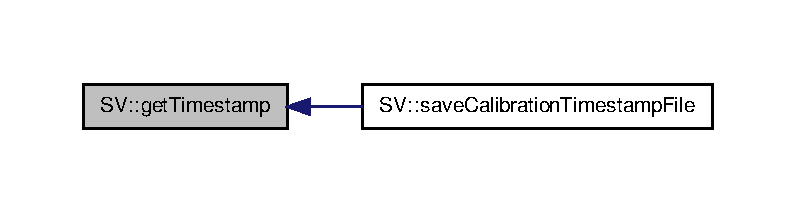
\includegraphics[width=350pt]{namespace_s_v_a9f7b63fd7ff59d018c9033a412abc4c0_icgraph}
\end{center}
\end{figure}


\hypertarget{namespace_s_v_a2eeee0cf678d9d481d3d3549b151a4a6}{\index{S\-V@{S\-V}!load\-Calibration\-Pattern\-File@{load\-Calibration\-Pattern\-File}}
\index{load\-Calibration\-Pattern\-File@{load\-Calibration\-Pattern\-File}!SV@{S\-V}}
\subsubsection[{load\-Calibration\-Pattern\-File}]{\setlength{\rightskip}{0pt plus 5cm}{\bf S\-V\-::\-Calibration\-Pattern} S\-V\-::load\-Calibration\-Pattern\-File (
\begin{DoxyParamCaption}
{}
\end{DoxyParamCaption}
)}}\label{namespace_s_v_a2eeee0cf678d9d481d3d3549b151a4a6}


Definition at line 85 of file Utility.\-cpp.



Here is the caller graph for this function\-:
\nopagebreak
\begin{figure}[H]
\begin{center}
\leavevmode
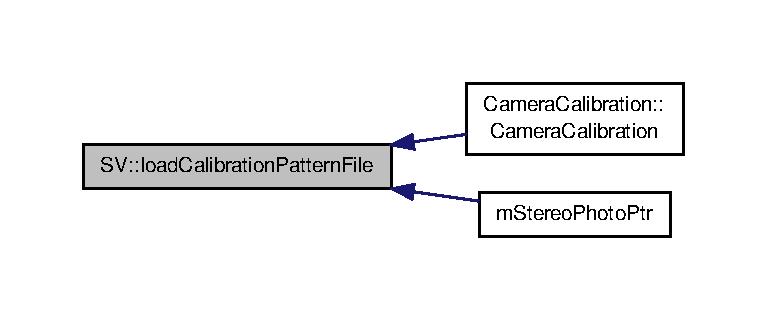
\includegraphics[width=350pt]{namespace_s_v_a2eeee0cf678d9d481d3d3549b151a4a6_icgraph}
\end{center}
\end{figure}


\hypertarget{namespace_s_v_ae32886e460af95f632f666beb6846946}{\index{S\-V@{S\-V}!load\-Calibration\-Timestamp\-File@{load\-Calibration\-Timestamp\-File}}
\index{load\-Calibration\-Timestamp\-File@{load\-Calibration\-Timestamp\-File}!SV@{S\-V}}
\subsubsection[{load\-Calibration\-Timestamp\-File}]{\setlength{\rightskip}{0pt plus 5cm}std\-::string S\-V\-::load\-Calibration\-Timestamp\-File (
\begin{DoxyParamCaption}
{}
\end{DoxyParamCaption}
)}}\label{namespace_s_v_ae32886e460af95f632f666beb6846946}


Definition at line 61 of file Utility.\-cpp.

\hypertarget{namespace_s_v_ad372136d1d33214cd8b7baa169fca11c}{\index{S\-V@{S\-V}!open\-C\-V\-Random\-Color@{open\-C\-V\-Random\-Color}}
\index{open\-C\-V\-Random\-Color@{open\-C\-V\-Random\-Color}!SV@{S\-V}}
\subsubsection[{open\-C\-V\-Random\-Color}]{\setlength{\rightskip}{0pt plus 5cm}cv\-::\-Scalar S\-V\-::open\-C\-V\-Random\-Color (
\begin{DoxyParamCaption}
\item[{cv\-::\-R\-N\-G \&}]{rng}
\end{DoxyParamCaption}
)}}\label{namespace_s_v_ad372136d1d33214cd8b7baa169fca11c}


Definition at line 152 of file Utility.\-cpp.



Here is the caller graph for this function\-:
\nopagebreak
\begin{figure}[H]
\begin{center}
\leavevmode
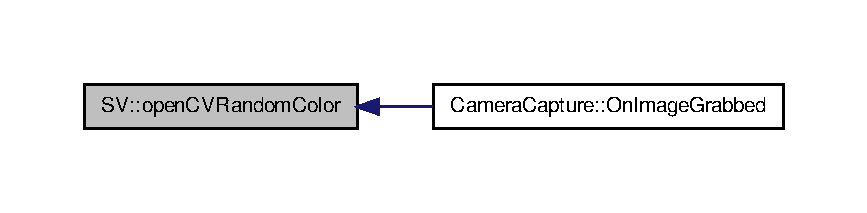
\includegraphics[width=350pt]{namespace_s_v_ad372136d1d33214cd8b7baa169fca11c_icgraph}
\end{center}
\end{figure}


\hypertarget{namespace_s_v_ae0b57b979ffff6071335b0e3af71d010}{\index{S\-V@{S\-V}!save\-Calibration\-Pattern\-File@{save\-Calibration\-Pattern\-File}}
\index{save\-Calibration\-Pattern\-File@{save\-Calibration\-Pattern\-File}!SV@{S\-V}}
\subsubsection[{save\-Calibration\-Pattern\-File}]{\setlength{\rightskip}{0pt plus 5cm}void S\-V\-::save\-Calibration\-Pattern\-File (
\begin{DoxyParamCaption}
\item[{unsigned int}]{w, }
\item[{unsigned int}]{h, }
\item[{float}]{s}
\end{DoxyParamCaption}
)}}\label{namespace_s_v_ae0b57b979ffff6071335b0e3af71d010}


Definition at line 103 of file Utility.\-cpp.

\hypertarget{namespace_s_v_a290f15aeacbb1347daab1947fd4f25a4}{\index{S\-V@{S\-V}!save\-Calibration\-Timestamp\-File@{save\-Calibration\-Timestamp\-File}}
\index{save\-Calibration\-Timestamp\-File@{save\-Calibration\-Timestamp\-File}!SV@{S\-V}}
\subsubsection[{save\-Calibration\-Timestamp\-File}]{\setlength{\rightskip}{0pt plus 5cm}void S\-V\-::save\-Calibration\-Timestamp\-File (
\begin{DoxyParamCaption}
{}
\end{DoxyParamCaption}
)}}\label{namespace_s_v_a290f15aeacbb1347daab1947fd4f25a4}


Definition at line 74 of file Utility.\-cpp.



Here is the call graph for this function\-:
\nopagebreak
\begin{figure}[H]
\begin{center}
\leavevmode
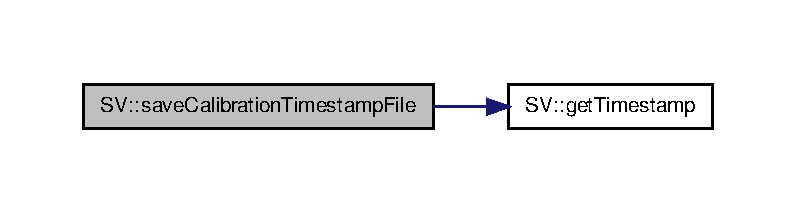
\includegraphics[width=350pt]{namespace_s_v_a290f15aeacbb1347daab1947fd4f25a4_cgraph}
\end{center}
\end{figure}




\subsection{Variable Documentation}
\hypertarget{namespace_s_v_a07b166ccd37fa68ea084cebb48a1f6f7}{\index{S\-V@{S\-V}!C\-A\-L\-I\-B\-R\-A\-T\-I\-O\-N\-\_\-\-B\-I\-N@{C\-A\-L\-I\-B\-R\-A\-T\-I\-O\-N\-\_\-\-B\-I\-N}}
\index{C\-A\-L\-I\-B\-R\-A\-T\-I\-O\-N\-\_\-\-B\-I\-N@{C\-A\-L\-I\-B\-R\-A\-T\-I\-O\-N\-\_\-\-B\-I\-N}!SV@{S\-V}}
\subsubsection[{C\-A\-L\-I\-B\-R\-A\-T\-I\-O\-N\-\_\-\-B\-I\-N}]{\setlength{\rightskip}{0pt plus 5cm}const std\-::string S\-V\-::\-C\-A\-L\-I\-B\-R\-A\-T\-I\-O\-N\-\_\-\-B\-I\-N = \char`\"{}Stereo\-Calibration\char`\"{}}}\label{namespace_s_v_a07b166ccd37fa68ea084cebb48a1f6f7}


Definition at line 28 of file Utility.\-cpp.

\hypertarget{namespace_s_v_a7eee3c30084ee151a5d8e793f448dfca}{\index{S\-V@{S\-V}!C\-A\-L\-I\-B\-R\-A\-T\-I\-O\-N\-\_\-\-I\-M\-A\-G\-E\-\_\-\-L\-E\-F\-T@{C\-A\-L\-I\-B\-R\-A\-T\-I\-O\-N\-\_\-\-I\-M\-A\-G\-E\-\_\-\-L\-E\-F\-T}}
\index{C\-A\-L\-I\-B\-R\-A\-T\-I\-O\-N\-\_\-\-I\-M\-A\-G\-E\-\_\-\-L\-E\-F\-T@{C\-A\-L\-I\-B\-R\-A\-T\-I\-O\-N\-\_\-\-I\-M\-A\-G\-E\-\_\-\-L\-E\-F\-T}!SV@{S\-V}}
\subsubsection[{C\-A\-L\-I\-B\-R\-A\-T\-I\-O\-N\-\_\-\-I\-M\-A\-G\-E\-\_\-\-L\-E\-F\-T}]{\setlength{\rightskip}{0pt plus 5cm}const std\-::string S\-V\-::\-C\-A\-L\-I\-B\-R\-A\-T\-I\-O\-N\-\_\-\-I\-M\-A\-G\-E\-\_\-\-L\-E\-F\-T = \char`\"{}left.\-ppm\char`\"{}}}\label{namespace_s_v_a7eee3c30084ee151a5d8e793f448dfca}


Definition at line 34 of file Utility.\-cpp.

\hypertarget{namespace_s_v_a6b93f40cb116005baad0fa89d5e3ded3}{\index{S\-V@{S\-V}!C\-A\-L\-I\-B\-R\-A\-T\-I\-O\-N\-\_\-\-I\-M\-A\-G\-E\-\_\-\-R\-I\-G\-H\-T@{C\-A\-L\-I\-B\-R\-A\-T\-I\-O\-N\-\_\-\-I\-M\-A\-G\-E\-\_\-\-R\-I\-G\-H\-T}}
\index{C\-A\-L\-I\-B\-R\-A\-T\-I\-O\-N\-\_\-\-I\-M\-A\-G\-E\-\_\-\-R\-I\-G\-H\-T@{C\-A\-L\-I\-B\-R\-A\-T\-I\-O\-N\-\_\-\-I\-M\-A\-G\-E\-\_\-\-R\-I\-G\-H\-T}!SV@{S\-V}}
\subsubsection[{C\-A\-L\-I\-B\-R\-A\-T\-I\-O\-N\-\_\-\-I\-M\-A\-G\-E\-\_\-\-R\-I\-G\-H\-T}]{\setlength{\rightskip}{0pt plus 5cm}const std\-::string S\-V\-::\-C\-A\-L\-I\-B\-R\-A\-T\-I\-O\-N\-\_\-\-I\-M\-A\-G\-E\-\_\-\-R\-I\-G\-H\-T = \char`\"{}right.\-ppm\char`\"{}}}\label{namespace_s_v_a6b93f40cb116005baad0fa89d5e3ded3}


Definition at line 35 of file Utility.\-cpp.

\hypertarget{namespace_s_v_a31f33ecf5d55099dbdcbf01cbdc8f85e}{\index{S\-V@{S\-V}!C\-A\-L\-I\-B\-R\-A\-T\-I\-O\-N\-\_\-\-I\-M\-A\-G\-E\-S\-\_\-\-F\-I\-L\-E@{C\-A\-L\-I\-B\-R\-A\-T\-I\-O\-N\-\_\-\-I\-M\-A\-G\-E\-S\-\_\-\-F\-I\-L\-E}}
\index{C\-A\-L\-I\-B\-R\-A\-T\-I\-O\-N\-\_\-\-I\-M\-A\-G\-E\-S\-\_\-\-F\-I\-L\-E@{C\-A\-L\-I\-B\-R\-A\-T\-I\-O\-N\-\_\-\-I\-M\-A\-G\-E\-S\-\_\-\-F\-I\-L\-E}!SV@{S\-V}}
\subsubsection[{C\-A\-L\-I\-B\-R\-A\-T\-I\-O\-N\-\_\-\-I\-M\-A\-G\-E\-S\-\_\-\-F\-I\-L\-E}]{\setlength{\rightskip}{0pt plus 5cm}const std\-::string S\-V\-::\-C\-A\-L\-I\-B\-R\-A\-T\-I\-O\-N\-\_\-\-I\-M\-A\-G\-E\-S\-\_\-\-F\-I\-L\-E = \char`\"{}Config/Calibration/list.\-txt\char`\"{}}}\label{namespace_s_v_a31f33ecf5d55099dbdcbf01cbdc8f85e}


Definition at line 32 of file Utility.\-cpp.

\hypertarget{namespace_s_v_aca9f280a6ae4110ddbfcb3db20c40931}{\index{S\-V@{S\-V}!C\-A\-L\-I\-B\-R\-A\-T\-I\-O\-N\-\_\-\-I\-M\-A\-G\-E\-S\-\_\-\-P\-A\-T\-H@{C\-A\-L\-I\-B\-R\-A\-T\-I\-O\-N\-\_\-\-I\-M\-A\-G\-E\-S\-\_\-\-P\-A\-T\-H}}
\index{C\-A\-L\-I\-B\-R\-A\-T\-I\-O\-N\-\_\-\-I\-M\-A\-G\-E\-S\-\_\-\-P\-A\-T\-H@{C\-A\-L\-I\-B\-R\-A\-T\-I\-O\-N\-\_\-\-I\-M\-A\-G\-E\-S\-\_\-\-P\-A\-T\-H}!SV@{S\-V}}
\subsubsection[{C\-A\-L\-I\-B\-R\-A\-T\-I\-O\-N\-\_\-\-I\-M\-A\-G\-E\-S\-\_\-\-P\-A\-T\-H}]{\setlength{\rightskip}{0pt plus 5cm}const std\-::string S\-V\-::\-C\-A\-L\-I\-B\-R\-A\-T\-I\-O\-N\-\_\-\-I\-M\-A\-G\-E\-S\-\_\-\-P\-A\-T\-H = \char`\"{}Config/Calibration/Images/\char`\"{}}}\label{namespace_s_v_aca9f280a6ae4110ddbfcb3db20c40931}


Definition at line 33 of file Utility.\-cpp.

\hypertarget{namespace_s_v_ab14088c3b114b4905a5064056e160576}{\index{S\-V@{S\-V}!C\-A\-L\-I\-B\-R\-A\-T\-I\-O\-N\-\_\-\-P\-A\-T\-T\-E\-R\-N\-\_\-\-F\-I\-L\-E@{C\-A\-L\-I\-B\-R\-A\-T\-I\-O\-N\-\_\-\-P\-A\-T\-T\-E\-R\-N\-\_\-\-F\-I\-L\-E}}
\index{C\-A\-L\-I\-B\-R\-A\-T\-I\-O\-N\-\_\-\-P\-A\-T\-T\-E\-R\-N\-\_\-\-F\-I\-L\-E@{C\-A\-L\-I\-B\-R\-A\-T\-I\-O\-N\-\_\-\-P\-A\-T\-T\-E\-R\-N\-\_\-\-F\-I\-L\-E}!SV@{S\-V}}
\subsubsection[{C\-A\-L\-I\-B\-R\-A\-T\-I\-O\-N\-\_\-\-P\-A\-T\-T\-E\-R\-N\-\_\-\-F\-I\-L\-E}]{\setlength{\rightskip}{0pt plus 5cm}const std\-::string S\-V\-::\-C\-A\-L\-I\-B\-R\-A\-T\-I\-O\-N\-\_\-\-P\-A\-T\-T\-E\-R\-N\-\_\-\-F\-I\-L\-E = \char`\"{}Config/Calibration/pattern.\-txt\char`\"{}}}\label{namespace_s_v_ab14088c3b114b4905a5064056e160576}


Definition at line 30 of file Utility.\-cpp.

\hypertarget{namespace_s_v_a25683376004000d485cf2c87db0f6b2a}{\index{S\-V@{S\-V}!C\-A\-L\-I\-B\-R\-A\-T\-I\-O\-N\-\_\-\-T\-I\-M\-E\-S\-T\-A\-M\-P\-\_\-\-F\-I\-L\-E@{C\-A\-L\-I\-B\-R\-A\-T\-I\-O\-N\-\_\-\-T\-I\-M\-E\-S\-T\-A\-M\-P\-\_\-\-F\-I\-L\-E}}
\index{C\-A\-L\-I\-B\-R\-A\-T\-I\-O\-N\-\_\-\-T\-I\-M\-E\-S\-T\-A\-M\-P\-\_\-\-F\-I\-L\-E@{C\-A\-L\-I\-B\-R\-A\-T\-I\-O\-N\-\_\-\-T\-I\-M\-E\-S\-T\-A\-M\-P\-\_\-\-F\-I\-L\-E}!SV@{S\-V}}
\subsubsection[{C\-A\-L\-I\-B\-R\-A\-T\-I\-O\-N\-\_\-\-T\-I\-M\-E\-S\-T\-A\-M\-P\-\_\-\-F\-I\-L\-E}]{\setlength{\rightskip}{0pt plus 5cm}const std\-::string S\-V\-::\-C\-A\-L\-I\-B\-R\-A\-T\-I\-O\-N\-\_\-\-T\-I\-M\-E\-S\-T\-A\-M\-P\-\_\-\-F\-I\-L\-E = \char`\"{}Config/Calibration/timestamp.\-txt\char`\"{}}}\label{namespace_s_v_a25683376004000d485cf2c87db0f6b2a}


Definition at line 29 of file Utility.\-cpp.

\hypertarget{namespace_s_v_a08efa5f4f7f6a650b132fe6ce146c7a6}{\index{S\-V@{S\-V}!C\-A\-L\-I\-B\-R\-A\-T\-I\-O\-N\-\_\-\-X\-M\-L\-\_\-\-F\-I\-L\-E\-S\-\_\-\-P\-A\-T\-H@{C\-A\-L\-I\-B\-R\-A\-T\-I\-O\-N\-\_\-\-X\-M\-L\-\_\-\-F\-I\-L\-E\-S\-\_\-\-P\-A\-T\-H}}
\index{C\-A\-L\-I\-B\-R\-A\-T\-I\-O\-N\-\_\-\-X\-M\-L\-\_\-\-F\-I\-L\-E\-S\-\_\-\-P\-A\-T\-H@{C\-A\-L\-I\-B\-R\-A\-T\-I\-O\-N\-\_\-\-X\-M\-L\-\_\-\-F\-I\-L\-E\-S\-\_\-\-P\-A\-T\-H}!SV@{S\-V}}
\subsubsection[{C\-A\-L\-I\-B\-R\-A\-T\-I\-O\-N\-\_\-\-X\-M\-L\-\_\-\-F\-I\-L\-E\-S\-\_\-\-P\-A\-T\-H}]{\setlength{\rightskip}{0pt plus 5cm}const std\-::string S\-V\-::\-C\-A\-L\-I\-B\-R\-A\-T\-I\-O\-N\-\_\-\-X\-M\-L\-\_\-\-F\-I\-L\-E\-S\-\_\-\-P\-A\-T\-H = \char`\"{}Config/Calibration/X\-M\-L\-Files/\char`\"{}}}\label{namespace_s_v_a08efa5f4f7f6a650b132fe6ce146c7a6}


Definition at line 31 of file Utility.\-cpp.

\hypertarget{namespace_s_v_aa00fc841744191453046361becae6ae6}{\index{S\-V@{S\-V}!C\-O\-N\-F\-I\-G\-U\-R\-A\-T\-I\-O\-N\-\_\-\-F\-I\-L\-E@{C\-O\-N\-F\-I\-G\-U\-R\-A\-T\-I\-O\-N\-\_\-\-F\-I\-L\-E}}
\index{C\-O\-N\-F\-I\-G\-U\-R\-A\-T\-I\-O\-N\-\_\-\-F\-I\-L\-E@{C\-O\-N\-F\-I\-G\-U\-R\-A\-T\-I\-O\-N\-\_\-\-F\-I\-L\-E}!SV@{S\-V}}
\subsubsection[{C\-O\-N\-F\-I\-G\-U\-R\-A\-T\-I\-O\-N\-\_\-\-F\-I\-L\-E}]{\setlength{\rightskip}{0pt plus 5cm}const char $\ast$ S\-V\-::\-C\-O\-N\-F\-I\-G\-U\-R\-A\-T\-I\-O\-N\-\_\-\-F\-I\-L\-E = \char`\"{}Config/Camera/default\-\_\-linux.\-pfs\char`\"{}}}\label{namespace_s_v_aa00fc841744191453046361becae6ae6}


Definition at line 17 of file Utility.\-cpp.

\hypertarget{namespace_s_v_ab43026f6f6ee1b8e5cc36194a2ea9e6b}{\index{S\-V@{S\-V}!E\-M\-U\-L\-A\-T\-E\-D\-\_\-\-C\-A\-M\-E\-R\-A@{E\-M\-U\-L\-A\-T\-E\-D\-\_\-\-C\-A\-M\-E\-R\-A}}
\index{E\-M\-U\-L\-A\-T\-E\-D\-\_\-\-C\-A\-M\-E\-R\-A@{E\-M\-U\-L\-A\-T\-E\-D\-\_\-\-C\-A\-M\-E\-R\-A}!SV@{S\-V}}
\subsubsection[{E\-M\-U\-L\-A\-T\-E\-D\-\_\-\-C\-A\-M\-E\-R\-A}]{\setlength{\rightskip}{0pt plus 5cm}const std\-::string S\-V\-::\-E\-M\-U\-L\-A\-T\-E\-D\-\_\-\-C\-A\-M\-E\-R\-A = \char`\"{}Emulation\char`\"{}}}\label{namespace_s_v_ab43026f6f6ee1b8e5cc36194a2ea9e6b}


Definition at line 41 of file Utility.\-cpp.

\hypertarget{namespace_s_v_a4a601cd489e8ca00c55bb2785c8bb5d9}{\index{S\-V@{S\-V}!E\-M\-U\-L\-A\-T\-E\-D\-\_\-\-I\-M\-A\-G\-E\-S\-\_\-\-F\-I\-L\-E@{E\-M\-U\-L\-A\-T\-E\-D\-\_\-\-I\-M\-A\-G\-E\-S\-\_\-\-F\-I\-L\-E}}
\index{E\-M\-U\-L\-A\-T\-E\-D\-\_\-\-I\-M\-A\-G\-E\-S\-\_\-\-F\-I\-L\-E@{E\-M\-U\-L\-A\-T\-E\-D\-\_\-\-I\-M\-A\-G\-E\-S\-\_\-\-F\-I\-L\-E}!SV@{S\-V}}
\subsubsection[{E\-M\-U\-L\-A\-T\-E\-D\-\_\-\-I\-M\-A\-G\-E\-S\-\_\-\-F\-I\-L\-E}]{\setlength{\rightskip}{0pt plus 5cm}const std\-::string S\-V\-::\-E\-M\-U\-L\-A\-T\-E\-D\-\_\-\-I\-M\-A\-G\-E\-S\-\_\-\-F\-I\-L\-E = \char`\"{}Config/Calibration/list\-\_\-emulation.\-txt\char`\"{}}}\label{namespace_s_v_a4a601cd489e8ca00c55bb2785c8bb5d9}


Definition at line 42 of file Utility.\-cpp.

\hypertarget{namespace_s_v_ab98fb68d38e7637f92d456f945dfd2ff}{\index{S\-V@{S\-V}!E\-M\-U\-L\-A\-T\-E\-D\-\_\-\-I\-M\-A\-G\-E\-S\-\_\-\-P\-A\-T\-H@{E\-M\-U\-L\-A\-T\-E\-D\-\_\-\-I\-M\-A\-G\-E\-S\-\_\-\-P\-A\-T\-H}}
\index{E\-M\-U\-L\-A\-T\-E\-D\-\_\-\-I\-M\-A\-G\-E\-S\-\_\-\-P\-A\-T\-H@{E\-M\-U\-L\-A\-T\-E\-D\-\_\-\-I\-M\-A\-G\-E\-S\-\_\-\-P\-A\-T\-H}!SV@{S\-V}}
\subsubsection[{E\-M\-U\-L\-A\-T\-E\-D\-\_\-\-I\-M\-A\-G\-E\-S\-\_\-\-P\-A\-T\-H}]{\setlength{\rightskip}{0pt plus 5cm}const std\-::string S\-V\-::\-E\-M\-U\-L\-A\-T\-E\-D\-\_\-\-I\-M\-A\-G\-E\-S\-\_\-\-P\-A\-T\-H = {\bf S\-V\-::\-C\-A\-L\-I\-B\-R\-A\-T\-I\-O\-N\-\_\-\-I\-M\-A\-G\-E\-S\-\_\-\-P\-A\-T\-H} + \char`\"{}Emulation/\char`\"{}}}\label{namespace_s_v_ab98fb68d38e7637f92d456f945dfd2ff}


Definition at line 43 of file Utility.\-cpp.

\hypertarget{namespace_s_v_abef27351d2e2c8b13783f080571edca8}{\index{S\-V@{S\-V}!E\-M\-U\-L\-A\-T\-I\-O\-N\-\_\-\-M\-O\-D\-E@{E\-M\-U\-L\-A\-T\-I\-O\-N\-\_\-\-M\-O\-D\-E}}
\index{E\-M\-U\-L\-A\-T\-I\-O\-N\-\_\-\-M\-O\-D\-E@{E\-M\-U\-L\-A\-T\-I\-O\-N\-\_\-\-M\-O\-D\-E}!SV@{S\-V}}
\subsubsection[{E\-M\-U\-L\-A\-T\-I\-O\-N\-\_\-\-M\-O\-D\-E}]{\setlength{\rightskip}{0pt plus 5cm}bool S\-V\-::\-E\-M\-U\-L\-A\-T\-I\-O\-N\-\_\-\-M\-O\-D\-E = false}}\label{namespace_s_v_abef27351d2e2c8b13783f080571edca8}


Definition at line 40 of file Utility.\-cpp.

\hypertarget{namespace_s_v_a91d9ea38d5f6a4803e3e94ad8c9a722a}{\index{S\-V@{S\-V}!F\-R\-A\-M\-E\-\_\-\-T\-R\-A\-N\-S\-M\-I\-S\-S\-I\-O\-N\-\_\-\-D\-E\-L\-A\-Y@{F\-R\-A\-M\-E\-\_\-\-T\-R\-A\-N\-S\-M\-I\-S\-S\-I\-O\-N\-\_\-\-D\-E\-L\-A\-Y}}
\index{F\-R\-A\-M\-E\-\_\-\-T\-R\-A\-N\-S\-M\-I\-S\-S\-I\-O\-N\-\_\-\-D\-E\-L\-A\-Y@{F\-R\-A\-M\-E\-\_\-\-T\-R\-A\-N\-S\-M\-I\-S\-S\-I\-O\-N\-\_\-\-D\-E\-L\-A\-Y}!SV@{S\-V}}
\subsubsection[{F\-R\-A\-M\-E\-\_\-\-T\-R\-A\-N\-S\-M\-I\-S\-S\-I\-O\-N\-\_\-\-D\-E\-L\-A\-Y}]{\setlength{\rightskip}{0pt plus 5cm}const int S\-V\-::\-F\-R\-A\-M\-E\-\_\-\-T\-R\-A\-N\-S\-M\-I\-S\-S\-I\-O\-N\-\_\-\-D\-E\-L\-A\-Y = 4096 + {\bf S\-V\-::\-M\-A\-I\-N\-\_\-\-L\-O\-O\-P\-\_\-\-I\-T\-E\-R\-A\-T\-I\-O\-N\-\_\-\-T\-I\-M\-E}}}\label{namespace_s_v_a91d9ea38d5f6a4803e3e94ad8c9a722a}


Definition at line 24 of file Utility.\-cpp.

\hypertarget{namespace_s_v_aa245d3d1f71d5a419cefdc42626b1c07}{\index{S\-V@{S\-V}!I\-N\-T\-E\-R\-\_\-\-P\-A\-C\-K\-E\-T\-\_\-\-D\-E\-L\-A\-Y@{I\-N\-T\-E\-R\-\_\-\-P\-A\-C\-K\-E\-T\-\_\-\-D\-E\-L\-A\-Y}}
\index{I\-N\-T\-E\-R\-\_\-\-P\-A\-C\-K\-E\-T\-\_\-\-D\-E\-L\-A\-Y@{I\-N\-T\-E\-R\-\_\-\-P\-A\-C\-K\-E\-T\-\_\-\-D\-E\-L\-A\-Y}!SV@{S\-V}}
\subsubsection[{I\-N\-T\-E\-R\-\_\-\-P\-A\-C\-K\-E\-T\-\_\-\-D\-E\-L\-A\-Y}]{\setlength{\rightskip}{0pt plus 5cm}const int S\-V\-::\-I\-N\-T\-E\-R\-\_\-\-P\-A\-C\-K\-E\-T\-\_\-\-D\-E\-L\-A\-Y = 8192}}\label{namespace_s_v_aa245d3d1f71d5a419cefdc42626b1c07}


Definition at line 22 of file Utility.\-cpp.

\hypertarget{namespace_s_v_aa04b6739e3012b22c033d003c26d5584}{\index{S\-V@{S\-V}!line\-Break@{line\-Break}}
\index{line\-Break@{line\-Break}!SV@{S\-V}}
\subsubsection[{line\-Break}]{\setlength{\rightskip}{0pt plus 5cm}const std\-::string S\-V\-::line\-Break = \char`\"{}================================\textbackslash{}n\char`\"{}}}\label{namespace_s_v_aa04b6739e3012b22c033d003c26d5584}


Definition at line 47 of file Utility.\-cpp.

\hypertarget{namespace_s_v_a778a8d19ba21816aca4e8ca6c2dcd4a2}{\index{S\-V@{S\-V}!M\-A\-I\-N\-\_\-\-L\-O\-O\-P\-\_\-\-I\-T\-E\-R\-A\-T\-I\-O\-N\-\_\-\-T\-I\-M\-E@{M\-A\-I\-N\-\_\-\-L\-O\-O\-P\-\_\-\-I\-T\-E\-R\-A\-T\-I\-O\-N\-\_\-\-T\-I\-M\-E}}
\index{M\-A\-I\-N\-\_\-\-L\-O\-O\-P\-\_\-\-I\-T\-E\-R\-A\-T\-I\-O\-N\-\_\-\-T\-I\-M\-E@{M\-A\-I\-N\-\_\-\-L\-O\-O\-P\-\_\-\-I\-T\-E\-R\-A\-T\-I\-O\-N\-\_\-\-T\-I\-M\-E}!SV@{S\-V}}
\subsubsection[{M\-A\-I\-N\-\_\-\-L\-O\-O\-P\-\_\-\-I\-T\-E\-R\-A\-T\-I\-O\-N\-\_\-\-T\-I\-M\-E}]{\setlength{\rightskip}{0pt plus 5cm}int S\-V\-::\-M\-A\-I\-N\-\_\-\-L\-O\-O\-P\-\_\-\-I\-T\-E\-R\-A\-T\-I\-O\-N\-\_\-\-T\-I\-M\-E = 0}}\label{namespace_s_v_a778a8d19ba21816aca4e8ca6c2dcd4a2}


Definition at line 20 of file Utility.\-cpp.

\hypertarget{namespace_s_v_aa2acf99b8a3b122f688769ef693c30ae}{\index{S\-V@{S\-V}!M\-A\-X\-\_\-\-N\-U\-M\-B\-E\-R\-\_\-\-O\-F\-\_\-\-C\-A\-M\-E\-R\-A\-S@{M\-A\-X\-\_\-\-N\-U\-M\-B\-E\-R\-\_\-\-O\-F\-\_\-\-C\-A\-M\-E\-R\-A\-S}}
\index{M\-A\-X\-\_\-\-N\-U\-M\-B\-E\-R\-\_\-\-O\-F\-\_\-\-C\-A\-M\-E\-R\-A\-S@{M\-A\-X\-\_\-\-N\-U\-M\-B\-E\-R\-\_\-\-O\-F\-\_\-\-C\-A\-M\-E\-R\-A\-S}!SV@{S\-V}}
\subsubsection[{M\-A\-X\-\_\-\-N\-U\-M\-B\-E\-R\-\_\-\-O\-F\-\_\-\-C\-A\-M\-E\-R\-A\-S}]{\setlength{\rightskip}{0pt plus 5cm}const int S\-V\-::\-M\-A\-X\-\_\-\-N\-U\-M\-B\-E\-R\-\_\-\-O\-F\-\_\-\-C\-A\-M\-E\-R\-A\-S = 2}}\label{namespace_s_v_aa2acf99b8a3b122f688769ef693c30ae}


Definition at line 15 of file Utility.\-cpp.

\hypertarget{namespace_s_v_af29adc97546d0aacc73089470104b7e6}{\index{S\-V@{S\-V}!N\-O\-T\-\_\-\-C\-A\-L\-I\-B\-R\-A\-T\-E\-D@{N\-O\-T\-\_\-\-C\-A\-L\-I\-B\-R\-A\-T\-E\-D}}
\index{N\-O\-T\-\_\-\-C\-A\-L\-I\-B\-R\-A\-T\-E\-D@{N\-O\-T\-\_\-\-C\-A\-L\-I\-B\-R\-A\-T\-E\-D}!SV@{S\-V}}
\subsubsection[{N\-O\-T\-\_\-\-C\-A\-L\-I\-B\-R\-A\-T\-E\-D}]{\setlength{\rightskip}{0pt plus 5cm}const std\-::string S\-V\-::\-N\-O\-T\-\_\-\-C\-A\-L\-I\-B\-R\-A\-T\-E\-D = \char`\"{}N\-O\-T\-\_\-\-C\-A\-L\-I\-B\-R\-A\-T\-E\-D\char`\"{}}}\label{namespace_s_v_af29adc97546d0aacc73089470104b7e6}


Definition at line 36 of file Utility.\-cpp.


\chapter{Class Documentation}
\hypertarget{class_application}{\section{Application Class Reference}
\label{class_application}\index{Application@{Application}}
}


{\ttfamily \#include $<$Application.\-hpp$>$}

\subsection*{Public Member Functions}
\begin{DoxyCompactItemize}
\item 
\hyperlink{class_application_afa8cc05ce6b6092be5ecdfdae44e05f8}{Application} ()
\item 
void \hyperlink{class_application_a68965449404743bf1add056784d6cf81}{run} ()
\end{DoxyCompactItemize}


\subsection{Detailed Description}


Definition at line 14 of file Application.\-hpp.



\subsection{Constructor \& Destructor Documentation}
\hypertarget{class_application_afa8cc05ce6b6092be5ecdfdae44e05f8}{\index{Application@{Application}!Application@{Application}}
\index{Application@{Application}!Application@{Application}}
\subsubsection[{Application}]{\setlength{\rightskip}{0pt plus 5cm}Application\-::\-Application (
\begin{DoxyParamCaption}
{}
\end{DoxyParamCaption}
)}}\label{class_application_afa8cc05ce6b6092be5ecdfdae44e05f8}


Definition at line 13 of file Application.\-cpp.



\subsection{Member Function Documentation}
\hypertarget{class_application_a68965449404743bf1add056784d6cf81}{\index{Application@{Application}!run@{run}}
\index{run@{run}!Application@{Application}}
\subsubsection[{run}]{\setlength{\rightskip}{0pt plus 5cm}void Application\-::run (
\begin{DoxyParamCaption}
{}
\end{DoxyParamCaption}
)}}\label{class_application_a68965449404743bf1add056784d6cf81}


Definition at line 28 of file Application.\-cpp.



Here is the caller graph for this function\-:
\nopagebreak
\begin{figure}[H]
\begin{center}
\leavevmode
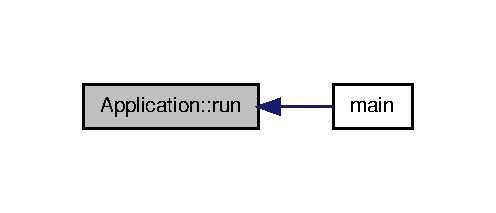
\includegraphics[width=238pt]{class_application_a68965449404743bf1add056784d6cf81_icgraph}
\end{center}
\end{figure}




The documentation for this class was generated from the following files\-:\begin{DoxyCompactItemize}
\item 
/home/gabriel/\-Templates/\-Stereo\-Vision/\-Include/\-S\-V/\hyperlink{_application_8hpp}{Application.\-hpp}\item 
/home/gabriel/\-Templates/\-Stereo\-Vision/\-Source/\hyperlink{_application_8cpp}{Application.\-cpp}\end{DoxyCompactItemize}

\hypertarget{struct_s_v_1_1_calibration_pattern}{\section{S\-V\-:\-:Calibration\-Pattern Struct Reference}
\label{struct_s_v_1_1_calibration_pattern}\index{S\-V\-::\-Calibration\-Pattern@{S\-V\-::\-Calibration\-Pattern}}
}


{\ttfamily \#include $<$Utility.\-hpp$>$}

\subsection*{Public Member Functions}
\begin{DoxyCompactItemize}
\item 
\hyperlink{struct_s_v_1_1_calibration_pattern_af5bda0ab3f29d5f00c733b00c764194b}{Calibration\-Pattern} (unsigned int corners\-Width, unsigned int corners\-Height, float square\-Size)
\end{DoxyCompactItemize}
\subsection*{Public Attributes}
\begin{DoxyCompactItemize}
\item 
unsigned int \hyperlink{struct_s_v_1_1_calibration_pattern_a99b723ddb247ba8a45bbae90f72992ee}{w}
\item 
unsigned int \hyperlink{struct_s_v_1_1_calibration_pattern_abcf472770054feb05d37291dbb7af10f}{h}
\item 
float \hyperlink{struct_s_v_1_1_calibration_pattern_a1a2f7fe30888c5f9bb8816d0809aedd3}{s}
\end{DoxyCompactItemize}


\subsection{Detailed Description}


Definition at line 32 of file Utility.\-hpp.



\subsection{Constructor \& Destructor Documentation}
\hypertarget{struct_s_v_1_1_calibration_pattern_af5bda0ab3f29d5f00c733b00c764194b}{\index{S\-V\-::\-Calibration\-Pattern@{S\-V\-::\-Calibration\-Pattern}!Calibration\-Pattern@{Calibration\-Pattern}}
\index{Calibration\-Pattern@{Calibration\-Pattern}!SV::CalibrationPattern@{S\-V\-::\-Calibration\-Pattern}}
\subsubsection[{Calibration\-Pattern}]{\setlength{\rightskip}{0pt plus 5cm}S\-V\-::\-Calibration\-Pattern\-::\-Calibration\-Pattern (
\begin{DoxyParamCaption}
\item[{unsigned int}]{corners\-Width, }
\item[{unsigned int}]{corners\-Height, }
\item[{float}]{square\-Size}
\end{DoxyParamCaption}
)\hspace{0.3cm}{\ttfamily [inline]}}}\label{struct_s_v_1_1_calibration_pattern_af5bda0ab3f29d5f00c733b00c764194b}


Definition at line 34 of file Utility.\-hpp.



\subsection{Member Data Documentation}
\hypertarget{struct_s_v_1_1_calibration_pattern_abcf472770054feb05d37291dbb7af10f}{\index{S\-V\-::\-Calibration\-Pattern@{S\-V\-::\-Calibration\-Pattern}!h@{h}}
\index{h@{h}!SV::CalibrationPattern@{S\-V\-::\-Calibration\-Pattern}}
\subsubsection[{h}]{\setlength{\rightskip}{0pt plus 5cm}unsigned int S\-V\-::\-Calibration\-Pattern\-::h}}\label{struct_s_v_1_1_calibration_pattern_abcf472770054feb05d37291dbb7af10f}


Definition at line 42 of file Utility.\-hpp.

\hypertarget{struct_s_v_1_1_calibration_pattern_a1a2f7fe30888c5f9bb8816d0809aedd3}{\index{S\-V\-::\-Calibration\-Pattern@{S\-V\-::\-Calibration\-Pattern}!s@{s}}
\index{s@{s}!SV::CalibrationPattern@{S\-V\-::\-Calibration\-Pattern}}
\subsubsection[{s}]{\setlength{\rightskip}{0pt plus 5cm}float S\-V\-::\-Calibration\-Pattern\-::s}}\label{struct_s_v_1_1_calibration_pattern_a1a2f7fe30888c5f9bb8816d0809aedd3}


Definition at line 43 of file Utility.\-hpp.

\hypertarget{struct_s_v_1_1_calibration_pattern_a99b723ddb247ba8a45bbae90f72992ee}{\index{S\-V\-::\-Calibration\-Pattern@{S\-V\-::\-Calibration\-Pattern}!w@{w}}
\index{w@{w}!SV::CalibrationPattern@{S\-V\-::\-Calibration\-Pattern}}
\subsubsection[{w}]{\setlength{\rightskip}{0pt plus 5cm}unsigned int S\-V\-::\-Calibration\-Pattern\-::w}}\label{struct_s_v_1_1_calibration_pattern_a99b723ddb247ba8a45bbae90f72992ee}


Definition at line 41 of file Utility.\-hpp.



The documentation for this struct was generated from the following file\-:\begin{DoxyCompactItemize}
\item 
/home/gabriel/\-Templates/\-Stereo\-Vision/\-Include/\-S\-V/\hyperlink{_utility_8hpp}{Utility.\-hpp}\end{DoxyCompactItemize}

\hypertarget{class_camera_calibration}{\section{Camera\-Calibration Class Reference}
\label{class_camera_calibration}\index{Camera\-Calibration@{Camera\-Calibration}}
}


{\ttfamily \#include $<$Camera\-Calibration.\-hpp$>$}



Inheritance diagram for Camera\-Calibration\-:
\nopagebreak
\begin{figure}[H]
\begin{center}
\leavevmode
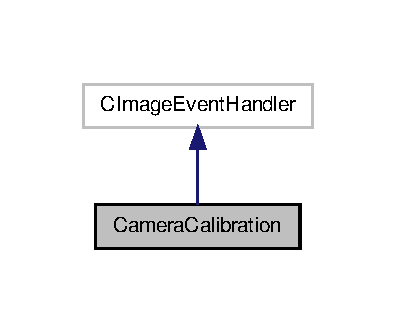
\includegraphics[width=190pt]{class_camera_calibration__inherit__graph}
\end{center}
\end{figure}


Collaboration diagram for Camera\-Calibration\-:
\nopagebreak
\begin{figure}[H]
\begin{center}
\leavevmode
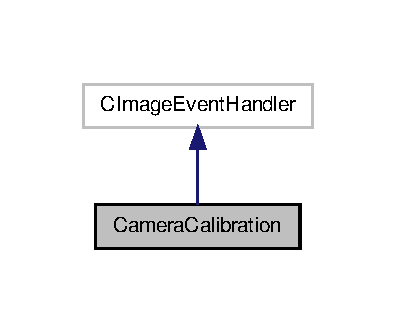
\includegraphics[width=190pt]{class_camera_calibration__coll__graph}
\end{center}
\end{figure}
\subsection*{Public Member Functions}
\begin{DoxyCompactItemize}
\item 
\hyperlink{class_camera_calibration_a9a5d8bd3ff591bdab35b05cdb6af879a}{Camera\-Calibration} (std\-::string camera\-Name, unsigned int $\ast$grab\-Count\-Ptr, std\-::ofstream $\ast$image\-List\-File\-Ptr)
\item 
virtual void \hyperlink{class_camera_calibration_a738936b0e792517f3f849e1a4504180b}{On\-Image\-Grabbed} (Pylon\-::\-C\-Instant\-Camera \&camera, const Pylon\-::\-C\-Grab\-Result\-Ptr \&grab\-Result\-Ptr)
\end{DoxyCompactItemize}


\subsection{Detailed Description}


Definition at line 19 of file Camera\-Calibration.\-hpp.



\subsection{Constructor \& Destructor Documentation}
\hypertarget{class_camera_calibration_a9a5d8bd3ff591bdab35b05cdb6af879a}{\index{Camera\-Calibration@{Camera\-Calibration}!Camera\-Calibration@{Camera\-Calibration}}
\index{Camera\-Calibration@{Camera\-Calibration}!CameraCalibration@{Camera\-Calibration}}
\subsubsection[{Camera\-Calibration}]{\setlength{\rightskip}{0pt plus 5cm}Camera\-Calibration\-::\-Camera\-Calibration (
\begin{DoxyParamCaption}
\item[{std\-::string}]{camera\-Name, }
\item[{unsigned int $\ast$}]{grab\-Count\-Ptr, }
\item[{std\-::ofstream $\ast$}]{image\-List\-File\-Ptr}
\end{DoxyParamCaption}
)}}\label{class_camera_calibration_a9a5d8bd3ff591bdab35b05cdb6af879a}


Definition at line 15 of file Camera\-Calibration.\-cpp.



Here is the call graph for this function\-:
\nopagebreak
\begin{figure}[H]
\begin{center}
\leavevmode
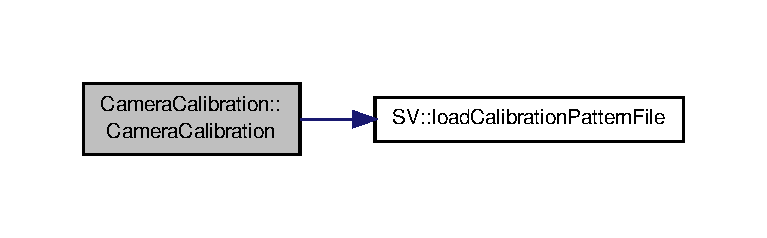
\includegraphics[width=350pt]{class_camera_calibration_a9a5d8bd3ff591bdab35b05cdb6af879a_cgraph}
\end{center}
\end{figure}




\subsection{Member Function Documentation}
\hypertarget{class_camera_calibration_a738936b0e792517f3f849e1a4504180b}{\index{Camera\-Calibration@{Camera\-Calibration}!On\-Image\-Grabbed@{On\-Image\-Grabbed}}
\index{On\-Image\-Grabbed@{On\-Image\-Grabbed}!CameraCalibration@{Camera\-Calibration}}
\subsubsection[{On\-Image\-Grabbed}]{\setlength{\rightskip}{0pt plus 5cm}void Camera\-Calibration\-::\-On\-Image\-Grabbed (
\begin{DoxyParamCaption}
\item[{Pylon\-::\-C\-Instant\-Camera \&}]{camera, }
\item[{const Pylon\-::\-C\-Grab\-Result\-Ptr \&}]{grab\-Result\-Ptr}
\end{DoxyParamCaption}
)\hspace{0.3cm}{\ttfamily [virtual]}}}\label{class_camera_calibration_a738936b0e792517f3f849e1a4504180b}


Definition at line 28 of file Camera\-Calibration.\-cpp.



The documentation for this class was generated from the following files\-:\begin{DoxyCompactItemize}
\item 
/home/gabriel/\-Templates/\-Stereo\-Vision/\-Include/\-S\-V/\hyperlink{_camera_calibration_8hpp}{Camera\-Calibration.\-hpp}\item 
/home/gabriel/\-Templates/\-Stereo\-Vision/\-Source/\hyperlink{_camera_calibration_8cpp}{Camera\-Calibration.\-cpp}\end{DoxyCompactItemize}

\hypertarget{class_camera_capture}{\section{Camera\-Capture Class Reference}
\label{class_camera_capture}\index{Camera\-Capture@{Camera\-Capture}}
}


{\ttfamily \#include $<$Camera\-Capture.\-hpp$>$}



Inheritance diagram for Camera\-Capture\-:
\nopagebreak
\begin{figure}[H]
\begin{center}
\leavevmode
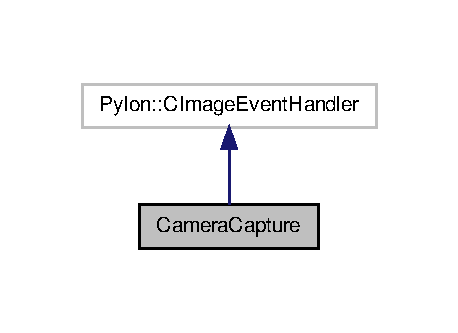
\includegraphics[width=220pt]{class_camera_capture__inherit__graph}
\end{center}
\end{figure}


Collaboration diagram for Camera\-Capture\-:
\nopagebreak
\begin{figure}[H]
\begin{center}
\leavevmode
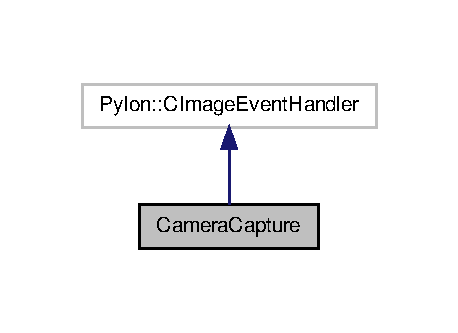
\includegraphics[width=220pt]{class_camera_capture__coll__graph}
\end{center}
\end{figure}
\subsection*{Public Member Functions}
\begin{DoxyCompactItemize}
\item 
\hyperlink{class_camera_capture_ace260c62593201ab93aa9bb5bb6b3e0e}{Camera\-Capture} (std\-::string camera\-Name, \hyperlink{struct_s_v_1_1_stereo_photo}{S\-V\-::\-Stereo\-Photo} $\ast$stereo\-Photo\-Ptr)
\item 
virtual void \hyperlink{class_camera_capture_a51f4f8a10ee4efbb2a15d5141ed7030c}{On\-Image\-Grabbed} (Pylon\-::\-C\-Instant\-Camera \&camera, const Pylon\-::\-C\-Grab\-Result\-Ptr \&grab\-Result\-Ptr)
\end{DoxyCompactItemize}


\subsection{Detailed Description}


Definition at line 31 of file Camera\-Capture.\-hpp.



\subsection{Constructor \& Destructor Documentation}
\hypertarget{class_camera_capture_ace260c62593201ab93aa9bb5bb6b3e0e}{\index{Camera\-Capture@{Camera\-Capture}!Camera\-Capture@{Camera\-Capture}}
\index{Camera\-Capture@{Camera\-Capture}!CameraCapture@{Camera\-Capture}}
\subsubsection[{Camera\-Capture}]{\setlength{\rightskip}{0pt plus 5cm}Camera\-Capture\-::\-Camera\-Capture (
\begin{DoxyParamCaption}
\item[{std\-::string}]{camera\-Name, }
\item[{{\bf S\-V\-::\-Stereo\-Photo} $\ast$}]{stereo\-Photo\-Ptr}
\end{DoxyParamCaption}
)}}\label{class_camera_capture_ace260c62593201ab93aa9bb5bb6b3e0e}


Definition at line 14 of file Camera\-Capture.\-cpp.



\subsection{Member Function Documentation}
\hypertarget{class_camera_capture_a51f4f8a10ee4efbb2a15d5141ed7030c}{\index{Camera\-Capture@{Camera\-Capture}!On\-Image\-Grabbed@{On\-Image\-Grabbed}}
\index{On\-Image\-Grabbed@{On\-Image\-Grabbed}!CameraCapture@{Camera\-Capture}}
\subsubsection[{On\-Image\-Grabbed}]{\setlength{\rightskip}{0pt plus 5cm}void Camera\-Capture\-::\-On\-Image\-Grabbed (
\begin{DoxyParamCaption}
\item[{Pylon\-::\-C\-Instant\-Camera \&}]{camera, }
\item[{const Pylon\-::\-C\-Grab\-Result\-Ptr \&}]{grab\-Result\-Ptr}
\end{DoxyParamCaption}
)\hspace{0.3cm}{\ttfamily [virtual]}}}\label{class_camera_capture_a51f4f8a10ee4efbb2a15d5141ed7030c}


Definition at line 43 of file Camera\-Capture.\-cpp.



Here is the call graph for this function\-:
\nopagebreak
\begin{figure}[H]
\begin{center}
\leavevmode
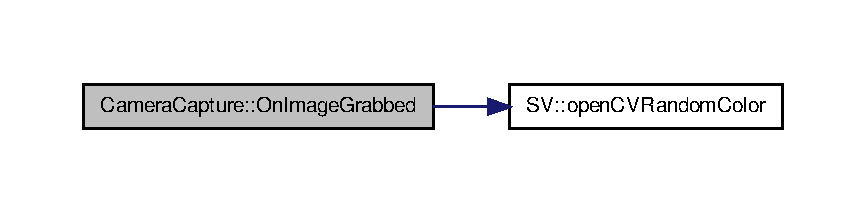
\includegraphics[width=350pt]{class_camera_capture_a51f4f8a10ee4efbb2a15d5141ed7030c_cgraph}
\end{center}
\end{figure}




The documentation for this class was generated from the following files\-:\begin{DoxyCompactItemize}
\item 
/home/gabriel/\-Templates/\-Stereo\-Vision/\-Include/\-S\-V/\hyperlink{_camera_capture_8hpp}{Camera\-Capture.\-hpp}\item 
/home/gabriel/\-Templates/\-Stereo\-Vision/\-Source/\hyperlink{_camera_capture_8cpp}{Camera\-Capture.\-cpp}\end{DoxyCompactItemize}

\hypertarget{class_camera_configuration}{\section{Camera\-Configuration Class Reference}
\label{class_camera_configuration}\index{Camera\-Configuration@{Camera\-Configuration}}
}


{\ttfamily \#include $<$Camera\-Configuration.\-hpp$>$}



Inheritance diagram for Camera\-Configuration\-:
\nopagebreak
\begin{figure}[H]
\begin{center}
\leavevmode
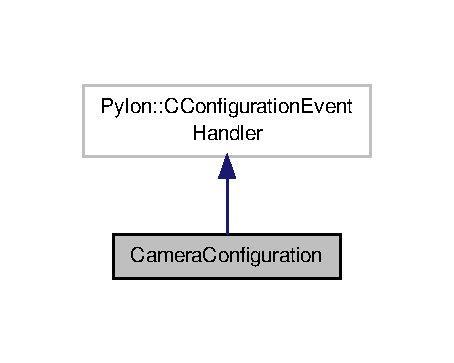
\includegraphics[width=218pt]{class_camera_configuration__inherit__graph}
\end{center}
\end{figure}


Collaboration diagram for Camera\-Configuration\-:
\nopagebreak
\begin{figure}[H]
\begin{center}
\leavevmode
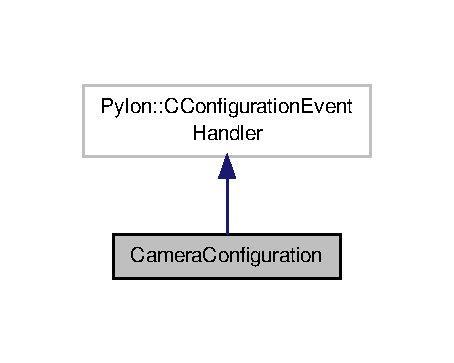
\includegraphics[width=218pt]{class_camera_configuration__coll__graph}
\end{center}
\end{figure}
\subsection*{Public Member Functions}
\begin{DoxyCompactItemize}
\item 
\hyperlink{class_camera_configuration_abb6adfa76a8054ca08609eac77297b73}{Camera\-Configuration} (const char $\ast$configuration\-File, const int inter\-Packet\-Delay, int frame\-Transmission\-Delay, std\-::string camera\-Name)
\item 
void \hyperlink{class_camera_configuration_aad7da12416c240adb4e4c0776e8483f0}{On\-Opened} (Pylon\-::\-C\-Instant\-Camera \&camera)
\item 
void \hyperlink{class_camera_configuration_ac542575f71d91aaec5f39c48603da019}{On\-Grab\-Started} (Pylon\-::\-C\-Instant\-Camera \&camera)
\end{DoxyCompactItemize}


\subsection{Detailed Description}


Definition at line 16 of file Camera\-Configuration.\-hpp.



\subsection{Constructor \& Destructor Documentation}
\hypertarget{class_camera_configuration_abb6adfa76a8054ca08609eac77297b73}{\index{Camera\-Configuration@{Camera\-Configuration}!Camera\-Configuration@{Camera\-Configuration}}
\index{Camera\-Configuration@{Camera\-Configuration}!CameraConfiguration@{Camera\-Configuration}}
\subsubsection[{Camera\-Configuration}]{\setlength{\rightskip}{0pt plus 5cm}Camera\-Configuration\-::\-Camera\-Configuration (
\begin{DoxyParamCaption}
\item[{const char $\ast$}]{configuration\-File, }
\item[{const int}]{inter\-Packet\-Delay, }
\item[{int}]{frame\-Transmission\-Delay, }
\item[{std\-::string}]{camera\-Name}
\end{DoxyParamCaption}
)}}\label{class_camera_configuration_abb6adfa76a8054ca08609eac77297b73}


Definition at line 12 of file Camera\-Configuration.\-cpp.



\subsection{Member Function Documentation}
\hypertarget{class_camera_configuration_ac542575f71d91aaec5f39c48603da019}{\index{Camera\-Configuration@{Camera\-Configuration}!On\-Grab\-Started@{On\-Grab\-Started}}
\index{On\-Grab\-Started@{On\-Grab\-Started}!CameraConfiguration@{Camera\-Configuration}}
\subsubsection[{On\-Grab\-Started}]{\setlength{\rightskip}{0pt plus 5cm}void Camera\-Configuration\-::\-On\-Grab\-Started (
\begin{DoxyParamCaption}
\item[{Pylon\-::\-C\-Instant\-Camera \&}]{camera}
\end{DoxyParamCaption}
)}}\label{class_camera_configuration_ac542575f71d91aaec5f39c48603da019}


Definition at line 48 of file Camera\-Configuration.\-cpp.

\hypertarget{class_camera_configuration_aad7da12416c240adb4e4c0776e8483f0}{\index{Camera\-Configuration@{Camera\-Configuration}!On\-Opened@{On\-Opened}}
\index{On\-Opened@{On\-Opened}!CameraConfiguration@{Camera\-Configuration}}
\subsubsection[{On\-Opened}]{\setlength{\rightskip}{0pt plus 5cm}void Camera\-Configuration\-::\-On\-Opened (
\begin{DoxyParamCaption}
\item[{Pylon\-::\-C\-Instant\-Camera \&}]{camera}
\end{DoxyParamCaption}
)}}\label{class_camera_configuration_aad7da12416c240adb4e4c0776e8483f0}


Definition at line 20 of file Camera\-Configuration.\-cpp.



The documentation for this class was generated from the following files\-:\begin{DoxyCompactItemize}
\item 
/home/gabriel/\-Templates/\-Stereo\-Vision/\-Include/\-S\-V/\hyperlink{_camera_configuration_8hpp}{Camera\-Configuration.\-hpp}\item 
/home/gabriel/\-Templates/\-Stereo\-Vision/\-Source/\hyperlink{_camera_configuration_8cpp}{Camera\-Configuration.\-cpp}\end{DoxyCompactItemize}

\hypertarget{struct_s_v_1_1_stereo_photo}{\section{S\-V\-:\-:Stereo\-Photo Struct Reference}
\label{struct_s_v_1_1_stereo_photo}\index{S\-V\-::\-Stereo\-Photo@{S\-V\-::\-Stereo\-Photo}}
}


{\ttfamily \#include $<$Utility.\-hpp$>$}

\subsection*{Public Attributes}
\begin{DoxyCompactItemize}
\item 
std\-::array$<$ std\-::string, 2 $>$ \hyperlink{struct_s_v_1_1_stereo_photo_ab9bf6406dbf4a4f03b1591b90841ccf6}{cameras}
\item 
std\-::pair$<$ cv\-::\-Mat, cv\-::\-Mat $>$ \hyperlink{struct_s_v_1_1_stereo_photo_ac54ead2c353e1a20bc15fc06b88f92ee}{mat\-Pair}
\end{DoxyCompactItemize}


\subsection{Detailed Description}


Definition at line 46 of file Utility.\-hpp.



\subsection{Member Data Documentation}
\hypertarget{struct_s_v_1_1_stereo_photo_ab9bf6406dbf4a4f03b1591b90841ccf6}{\index{S\-V\-::\-Stereo\-Photo@{S\-V\-::\-Stereo\-Photo}!cameras@{cameras}}
\index{cameras@{cameras}!SV::StereoPhoto@{S\-V\-::\-Stereo\-Photo}}
\subsubsection[{cameras}]{\setlength{\rightskip}{0pt plus 5cm}std\-::array$<$std\-::string, 2$>$ S\-V\-::\-Stereo\-Photo\-::cameras}}\label{struct_s_v_1_1_stereo_photo_ab9bf6406dbf4a4f03b1591b90841ccf6}


Definition at line 48 of file Utility.\-hpp.

\hypertarget{struct_s_v_1_1_stereo_photo_ac54ead2c353e1a20bc15fc06b88f92ee}{\index{S\-V\-::\-Stereo\-Photo@{S\-V\-::\-Stereo\-Photo}!mat\-Pair@{mat\-Pair}}
\index{mat\-Pair@{mat\-Pair}!SV::StereoPhoto@{S\-V\-::\-Stereo\-Photo}}
\subsubsection[{mat\-Pair}]{\setlength{\rightskip}{0pt plus 5cm}std\-::pair$<$cv\-::\-Mat, cv\-::\-Mat$>$ S\-V\-::\-Stereo\-Photo\-::mat\-Pair}}\label{struct_s_v_1_1_stereo_photo_ac54ead2c353e1a20bc15fc06b88f92ee}


Definition at line 49 of file Utility.\-hpp.



The documentation for this struct was generated from the following file\-:\begin{DoxyCompactItemize}
\item 
/home/gabriel/\-Templates/\-Stereo\-Vision/\-Include/\-S\-V/\hyperlink{_utility_8hpp}{Utility.\-hpp}\end{DoxyCompactItemize}

\chapter{File Documentation}
\hypertarget{_c_make_c_compiler_id_8c}{\section{/home/gabriel/\-Templates/\-Stereo\-Vision/\-Bin/\-C\-Make\-Files/2.8.11.2/\-Compiler\-Id\-C/\-C\-Make\-C\-Compiler\-Id.c File Reference}
\label{_c_make_c_compiler_id_8c}\index{/home/gabriel/\-Templates/\-Stereo\-Vision/\-Bin/\-C\-Make\-Files/2.\-8.\-11.\-2/\-Compiler\-Id\-C/\-C\-Make\-C\-Compiler\-Id.\-c@{/home/gabriel/\-Templates/\-Stereo\-Vision/\-Bin/\-C\-Make\-Files/2.\-8.\-11.\-2/\-Compiler\-Id\-C/\-C\-Make\-C\-Compiler\-Id.\-c}}
}
\subsection*{Macros}
\begin{DoxyCompactItemize}
\item 
\#define \hyperlink{_c_make_c_compiler_id_8c_a81dee0709ded976b2e0319239f72d174}{C\-O\-M\-P\-I\-L\-E\-R\-\_\-\-I\-D}~\char`\"{}\char`\"{}
\item 
\#define \hyperlink{_c_make_c_compiler_id_8c_adbc5372f40838899018fadbc89bd588b}{P\-L\-A\-T\-F\-O\-R\-M\-\_\-\-I\-D}~\char`\"{}\char`\"{}
\item 
\#define \hyperlink{_c_make_c_compiler_id_8c_aba35d0d200deaeb06aee95ca297acb28}{A\-R\-C\-H\-I\-T\-E\-C\-T\-U\-R\-E\-\_\-\-I\-D}~\char`\"{}\char`\"{}
\item 
\#define \hyperlink{_c_make_c_compiler_id_8c_ad1280362da42492bbc11aa78cbf776ad}{D\-E\-C}(n)
\item 
\#define \hyperlink{_c_make_c_compiler_id_8c_a46d5d95daa1bef867bd0179594310ed5}{H\-E\-X}(n)
\end{DoxyCompactItemize}
\subsection*{Functions}
\begin{DoxyCompactItemize}
\item 
int \hyperlink{_c_make_c_compiler_id_8c_a0ddf1224851353fc92bfbff6f499fa97}{main} (int argc, char $\ast$argv\mbox{[}$\,$\mbox{]})
\end{DoxyCompactItemize}
\subsection*{Variables}
\begin{DoxyCompactItemize}
\item 
char const $\ast$ \hyperlink{_c_make_c_compiler_id_8c_a4b0efeb7a5d59313986b3a0390f050f6}{info\-\_\-compiler} = \char`\"{}I\-N\-F\-O\char`\"{} \char`\"{}\-:\char`\"{} \char`\"{}compiler\mbox{[}\char`\"{} C\-O\-M\-P\-I\-L\-E\-R\-\_\-\-I\-D \char`\"{}\mbox{]}\char`\"{}
\item 
char const $\ast$ \hyperlink{_c_make_c_compiler_id_8c_a2321403dee54ee23f0c2fa849c60f7d4}{info\-\_\-platform} = \char`\"{}I\-N\-F\-O\char`\"{} \char`\"{}\-:\char`\"{} \char`\"{}platform\mbox{[}\char`\"{} P\-L\-A\-T\-F\-O\-R\-M\-\_\-\-I\-D \char`\"{}\mbox{]}\char`\"{}
\item 
char const $\ast$ \hyperlink{_c_make_c_compiler_id_8c_a59647e99d304ed33b15cb284c27ed391}{info\-\_\-arch} = \char`\"{}I\-N\-F\-O\char`\"{} \char`\"{}\-:\char`\"{} \char`\"{}arch\mbox{[}\char`\"{} A\-R\-C\-H\-I\-T\-E\-C\-T\-U\-R\-E\-\_\-\-I\-D \char`\"{}\mbox{]}\char`\"{}
\end{DoxyCompactItemize}


\subsection{Macro Definition Documentation}
\hypertarget{_c_make_c_compiler_id_8c_aba35d0d200deaeb06aee95ca297acb28}{\index{C\-Make\-C\-Compiler\-Id.\-c@{C\-Make\-C\-Compiler\-Id.\-c}!A\-R\-C\-H\-I\-T\-E\-C\-T\-U\-R\-E\-\_\-\-I\-D@{A\-R\-C\-H\-I\-T\-E\-C\-T\-U\-R\-E\-\_\-\-I\-D}}
\index{A\-R\-C\-H\-I\-T\-E\-C\-T\-U\-R\-E\-\_\-\-I\-D@{A\-R\-C\-H\-I\-T\-E\-C\-T\-U\-R\-E\-\_\-\-I\-D}!CMakeCCompilerId.c@{C\-Make\-C\-Compiler\-Id.\-c}}
\subsubsection[{A\-R\-C\-H\-I\-T\-E\-C\-T\-U\-R\-E\-\_\-\-I\-D}]{\setlength{\rightskip}{0pt plus 5cm}\#define A\-R\-C\-H\-I\-T\-E\-C\-T\-U\-R\-E\-\_\-\-I\-D~\char`\"{}\char`\"{}}}\label{_c_make_c_compiler_id_8c_aba35d0d200deaeb06aee95ca297acb28}


Definition at line 321 of file C\-Make\-C\-Compiler\-Id.\-c.

\hypertarget{_c_make_c_compiler_id_8c_a81dee0709ded976b2e0319239f72d174}{\index{C\-Make\-C\-Compiler\-Id.\-c@{C\-Make\-C\-Compiler\-Id.\-c}!C\-O\-M\-P\-I\-L\-E\-R\-\_\-\-I\-D@{C\-O\-M\-P\-I\-L\-E\-R\-\_\-\-I\-D}}
\index{C\-O\-M\-P\-I\-L\-E\-R\-\_\-\-I\-D@{C\-O\-M\-P\-I\-L\-E\-R\-\_\-\-I\-D}!CMakeCCompilerId.c@{C\-Make\-C\-Compiler\-Id.\-c}}
\subsubsection[{C\-O\-M\-P\-I\-L\-E\-R\-\_\-\-I\-D}]{\setlength{\rightskip}{0pt plus 5cm}\#define C\-O\-M\-P\-I\-L\-E\-R\-\_\-\-I\-D~\char`\"{}\char`\"{}}}\label{_c_make_c_compiler_id_8c_a81dee0709ded976b2e0319239f72d174}


Definition at line 201 of file C\-Make\-C\-Compiler\-Id.\-c.

\hypertarget{_c_make_c_compiler_id_8c_ad1280362da42492bbc11aa78cbf776ad}{\index{C\-Make\-C\-Compiler\-Id.\-c@{C\-Make\-C\-Compiler\-Id.\-c}!D\-E\-C@{D\-E\-C}}
\index{D\-E\-C@{D\-E\-C}!CMakeCCompilerId.c@{C\-Make\-C\-Compiler\-Id.\-c}}
\subsubsection[{D\-E\-C}]{\setlength{\rightskip}{0pt plus 5cm}\#define D\-E\-C(
\begin{DoxyParamCaption}
\item[{}]{n}
\end{DoxyParamCaption}
)}}\label{_c_make_c_compiler_id_8c_ad1280362da42492bbc11aa78cbf776ad}
{\bfseries Value\-:}
\begin{DoxyCode}
(\textcolor{charliteral}{'0'} + (((n) / 10000000)%10)), \(\backslash\)
  (\textcolor{charliteral}{'0'} + (((n) / 1000000)%10)),  \(\backslash\)
  (\textcolor{charliteral}{'0'} + (((n) / 100000)%10)),   \(\backslash\)
  (\textcolor{charliteral}{'0'} + (((n) / 10000)%10)),    \(\backslash\)
  (\textcolor{charliteral}{'0'} + (((n) / 1000)%10)),     \(\backslash\)
  (\textcolor{charliteral}{'0'} + (((n) / 100)%10)),      \(\backslash\)
  (\textcolor{charliteral}{'0'} + (((n) / 10)%10)),       \(\backslash\)
  (\textcolor{charliteral}{'0'} +  ((n) % 10))
\end{DoxyCode}


Definition at line 325 of file C\-Make\-C\-Compiler\-Id.\-c.

\hypertarget{_c_make_c_compiler_id_8c_a46d5d95daa1bef867bd0179594310ed5}{\index{C\-Make\-C\-Compiler\-Id.\-c@{C\-Make\-C\-Compiler\-Id.\-c}!H\-E\-X@{H\-E\-X}}
\index{H\-E\-X@{H\-E\-X}!CMakeCCompilerId.c@{C\-Make\-C\-Compiler\-Id.\-c}}
\subsubsection[{H\-E\-X}]{\setlength{\rightskip}{0pt plus 5cm}\#define H\-E\-X(
\begin{DoxyParamCaption}
\item[{}]{n}
\end{DoxyParamCaption}
)}}\label{_c_make_c_compiler_id_8c_a46d5d95daa1bef867bd0179594310ed5}
{\bfseries Value\-:}
\begin{DoxyCode}
(\textcolor{charliteral}{'0'} + ((n)>>28 & 0xF)), \(\backslash\)
  (\textcolor{charliteral}{'0'} + ((n)>>24 & 0xF)), \(\backslash\)
  (\textcolor{charliteral}{'0'} + ((n)>>20 & 0xF)), \(\backslash\)
  (\textcolor{charliteral}{'0'} + ((n)>>16 & 0xF)), \(\backslash\)
  (\textcolor{charliteral}{'0'} + ((n)>>12 & 0xF)), \(\backslash\)
  (\textcolor{charliteral}{'0'} + ((n)>>8  & 0xF)), \(\backslash\)
  (\textcolor{charliteral}{'0'} + ((n)>>4  & 0xF)), \(\backslash\)
  (\textcolor{charliteral}{'0'} + ((n)     & 0xF))
\end{DoxyCode}


Definition at line 336 of file C\-Make\-C\-Compiler\-Id.\-c.

\hypertarget{_c_make_c_compiler_id_8c_adbc5372f40838899018fadbc89bd588b}{\index{C\-Make\-C\-Compiler\-Id.\-c@{C\-Make\-C\-Compiler\-Id.\-c}!P\-L\-A\-T\-F\-O\-R\-M\-\_\-\-I\-D@{P\-L\-A\-T\-F\-O\-R\-M\-\_\-\-I\-D}}
\index{P\-L\-A\-T\-F\-O\-R\-M\-\_\-\-I\-D@{P\-L\-A\-T\-F\-O\-R\-M\-\_\-\-I\-D}!CMakeCCompilerId.c@{C\-Make\-C\-Compiler\-Id.\-c}}
\subsubsection[{P\-L\-A\-T\-F\-O\-R\-M\-\_\-\-I\-D}]{\setlength{\rightskip}{0pt plus 5cm}\#define P\-L\-A\-T\-F\-O\-R\-M\-\_\-\-I\-D~\char`\"{}\char`\"{}}}\label{_c_make_c_compiler_id_8c_adbc5372f40838899018fadbc89bd588b}


Definition at line 288 of file C\-Make\-C\-Compiler\-Id.\-c.



\subsection{Function Documentation}
\hypertarget{_c_make_c_compiler_id_8c_a0ddf1224851353fc92bfbff6f499fa97}{\index{C\-Make\-C\-Compiler\-Id.\-c@{C\-Make\-C\-Compiler\-Id.\-c}!main@{main}}
\index{main@{main}!CMakeCCompilerId.c@{C\-Make\-C\-Compiler\-Id.\-c}}
\subsubsection[{main}]{\setlength{\rightskip}{0pt plus 5cm}int main (
\begin{DoxyParamCaption}
\item[{int}]{argc, }
\item[{char $\ast$}]{argv\mbox{[}$\,$\mbox{]}}
\end{DoxyParamCaption}
)}}\label{_c_make_c_compiler_id_8c_a0ddf1224851353fc92bfbff6f499fa97}


Definition at line 378 of file C\-Make\-C\-Compiler\-Id.\-c.



\subsection{Variable Documentation}
\hypertarget{_c_make_c_compiler_id_8c_a59647e99d304ed33b15cb284c27ed391}{\index{C\-Make\-C\-Compiler\-Id.\-c@{C\-Make\-C\-Compiler\-Id.\-c}!info\-\_\-arch@{info\-\_\-arch}}
\index{info\-\_\-arch@{info\-\_\-arch}!CMakeCCompilerId.c@{C\-Make\-C\-Compiler\-Id.\-c}}
\subsubsection[{info\-\_\-arch}]{\setlength{\rightskip}{0pt plus 5cm}char const$\ast$ info\-\_\-arch = \char`\"{}I\-N\-F\-O\char`\"{} \char`\"{}\-:\char`\"{} \char`\"{}arch\mbox{[}\char`\"{} A\-R\-C\-H\-I\-T\-E\-C\-T\-U\-R\-E\-\_\-\-I\-D \char`\"{}\mbox{]}\char`\"{}}}\label{_c_make_c_compiler_id_8c_a59647e99d304ed33b15cb284c27ed391}


Definition at line 369 of file C\-Make\-C\-Compiler\-Id.\-c.

\hypertarget{_c_make_c_compiler_id_8c_a4b0efeb7a5d59313986b3a0390f050f6}{\index{C\-Make\-C\-Compiler\-Id.\-c@{C\-Make\-C\-Compiler\-Id.\-c}!info\-\_\-compiler@{info\-\_\-compiler}}
\index{info\-\_\-compiler@{info\-\_\-compiler}!CMakeCCompilerId.c@{C\-Make\-C\-Compiler\-Id.\-c}}
\subsubsection[{info\-\_\-compiler}]{\setlength{\rightskip}{0pt plus 5cm}char const$\ast$ info\-\_\-compiler = \char`\"{}I\-N\-F\-O\char`\"{} \char`\"{}\-:\char`\"{} \char`\"{}compiler\mbox{[}\char`\"{} C\-O\-M\-P\-I\-L\-E\-R\-\_\-\-I\-D \char`\"{}\mbox{]}\char`\"{}}}\label{_c_make_c_compiler_id_8c_a4b0efeb7a5d59313986b3a0390f050f6}


Definition at line 209 of file C\-Make\-C\-Compiler\-Id.\-c.

\hypertarget{_c_make_c_compiler_id_8c_a2321403dee54ee23f0c2fa849c60f7d4}{\index{C\-Make\-C\-Compiler\-Id.\-c@{C\-Make\-C\-Compiler\-Id.\-c}!info\-\_\-platform@{info\-\_\-platform}}
\index{info\-\_\-platform@{info\-\_\-platform}!CMakeCCompilerId.c@{C\-Make\-C\-Compiler\-Id.\-c}}
\subsubsection[{info\-\_\-platform}]{\setlength{\rightskip}{0pt plus 5cm}char const$\ast$ info\-\_\-platform = \char`\"{}I\-N\-F\-O\char`\"{} \char`\"{}\-:\char`\"{} \char`\"{}platform\mbox{[}\char`\"{} P\-L\-A\-T\-F\-O\-R\-M\-\_\-\-I\-D \char`\"{}\mbox{]}\char`\"{}}}\label{_c_make_c_compiler_id_8c_a2321403dee54ee23f0c2fa849c60f7d4}


Definition at line 368 of file C\-Make\-C\-Compiler\-Id.\-c.


\hypertarget{_c_make_c_x_x_compiler_id_8cpp}{\section{/home/gabriel/\-Templates/\-Stereo\-Vision/\-Bin/\-C\-Make\-Files/2.8.11.2/\-Compiler\-Id\-C\-X\-X/\-C\-Make\-C\-X\-X\-Compiler\-Id.cpp File Reference}
\label{_c_make_c_x_x_compiler_id_8cpp}\index{/home/gabriel/\-Templates/\-Stereo\-Vision/\-Bin/\-C\-Make\-Files/2.\-8.\-11.\-2/\-Compiler\-Id\-C\-X\-X/\-C\-Make\-C\-X\-X\-Compiler\-Id.\-cpp@{/home/gabriel/\-Templates/\-Stereo\-Vision/\-Bin/\-C\-Make\-Files/2.\-8.\-11.\-2/\-Compiler\-Id\-C\-X\-X/\-C\-Make\-C\-X\-X\-Compiler\-Id.\-cpp}}
}
\subsection*{Macros}
\begin{DoxyCompactItemize}
\item 
\#define \hyperlink{_c_make_c_x_x_compiler_id_8cpp_a81dee0709ded976b2e0319239f72d174}{C\-O\-M\-P\-I\-L\-E\-R\-\_\-\-I\-D}~\char`\"{}\char`\"{}
\item 
\#define \hyperlink{_c_make_c_x_x_compiler_id_8cpp_adbc5372f40838899018fadbc89bd588b}{P\-L\-A\-T\-F\-O\-R\-M\-\_\-\-I\-D}~\char`\"{}\char`\"{}
\item 
\#define \hyperlink{_c_make_c_x_x_compiler_id_8cpp_aba35d0d200deaeb06aee95ca297acb28}{A\-R\-C\-H\-I\-T\-E\-C\-T\-U\-R\-E\-\_\-\-I\-D}~\char`\"{}\char`\"{}
\item 
\#define \hyperlink{_c_make_c_x_x_compiler_id_8cpp_ad1280362da42492bbc11aa78cbf776ad}{D\-E\-C}(n)
\item 
\#define \hyperlink{_c_make_c_x_x_compiler_id_8cpp_a46d5d95daa1bef867bd0179594310ed5}{H\-E\-X}(n)
\end{DoxyCompactItemize}
\subsection*{Functions}
\begin{DoxyCompactItemize}
\item 
int \hyperlink{_c_make_c_x_x_compiler_id_8cpp_a0ddf1224851353fc92bfbff6f499fa97}{main} (int argc, char $\ast$argv\mbox{[}$\,$\mbox{]})
\end{DoxyCompactItemize}
\subsection*{Variables}
\begin{DoxyCompactItemize}
\item 
char const $\ast$ \hyperlink{_c_make_c_x_x_compiler_id_8cpp_a4b0efeb7a5d59313986b3a0390f050f6}{info\-\_\-compiler} = \char`\"{}I\-N\-F\-O\char`\"{} \char`\"{}\-:\char`\"{} \char`\"{}compiler\mbox{[}\char`\"{} C\-O\-M\-P\-I\-L\-E\-R\-\_\-\-I\-D \char`\"{}\mbox{]}\char`\"{}
\item 
char const $\ast$ \hyperlink{_c_make_c_x_x_compiler_id_8cpp_a2321403dee54ee23f0c2fa849c60f7d4}{info\-\_\-platform} = \char`\"{}I\-N\-F\-O\char`\"{} \char`\"{}\-:\char`\"{} \char`\"{}platform\mbox{[}\char`\"{} P\-L\-A\-T\-F\-O\-R\-M\-\_\-\-I\-D \char`\"{}\mbox{]}\char`\"{}
\item 
char const $\ast$ \hyperlink{_c_make_c_x_x_compiler_id_8cpp_a59647e99d304ed33b15cb284c27ed391}{info\-\_\-arch} = \char`\"{}I\-N\-F\-O\char`\"{} \char`\"{}\-:\char`\"{} \char`\"{}arch\mbox{[}\char`\"{} A\-R\-C\-H\-I\-T\-E\-C\-T\-U\-R\-E\-\_\-\-I\-D \char`\"{}\mbox{]}\char`\"{}
\end{DoxyCompactItemize}


\subsection{Macro Definition Documentation}
\hypertarget{_c_make_c_x_x_compiler_id_8cpp_aba35d0d200deaeb06aee95ca297acb28}{\index{C\-Make\-C\-X\-X\-Compiler\-Id.\-cpp@{C\-Make\-C\-X\-X\-Compiler\-Id.\-cpp}!A\-R\-C\-H\-I\-T\-E\-C\-T\-U\-R\-E\-\_\-\-I\-D@{A\-R\-C\-H\-I\-T\-E\-C\-T\-U\-R\-E\-\_\-\-I\-D}}
\index{A\-R\-C\-H\-I\-T\-E\-C\-T\-U\-R\-E\-\_\-\-I\-D@{A\-R\-C\-H\-I\-T\-E\-C\-T\-U\-R\-E\-\_\-\-I\-D}!CMakeCXXCompilerId.cpp@{C\-Make\-C\-X\-X\-Compiler\-Id.\-cpp}}
\subsubsection[{A\-R\-C\-H\-I\-T\-E\-C\-T\-U\-R\-E\-\_\-\-I\-D}]{\setlength{\rightskip}{0pt plus 5cm}\#define A\-R\-C\-H\-I\-T\-E\-C\-T\-U\-R\-E\-\_\-\-I\-D~\char`\"{}\char`\"{}}}\label{_c_make_c_x_x_compiler_id_8cpp_aba35d0d200deaeb06aee95ca297acb28}


Definition at line 308 of file C\-Make\-C\-X\-X\-Compiler\-Id.\-cpp.

\hypertarget{_c_make_c_x_x_compiler_id_8cpp_a81dee0709ded976b2e0319239f72d174}{\index{C\-Make\-C\-X\-X\-Compiler\-Id.\-cpp@{C\-Make\-C\-X\-X\-Compiler\-Id.\-cpp}!C\-O\-M\-P\-I\-L\-E\-R\-\_\-\-I\-D@{C\-O\-M\-P\-I\-L\-E\-R\-\_\-\-I\-D}}
\index{C\-O\-M\-P\-I\-L\-E\-R\-\_\-\-I\-D@{C\-O\-M\-P\-I\-L\-E\-R\-\_\-\-I\-D}!CMakeCXXCompilerId.cpp@{C\-Make\-C\-X\-X\-Compiler\-Id.\-cpp}}
\subsubsection[{C\-O\-M\-P\-I\-L\-E\-R\-\_\-\-I\-D}]{\setlength{\rightskip}{0pt plus 5cm}\#define C\-O\-M\-P\-I\-L\-E\-R\-\_\-\-I\-D~\char`\"{}\char`\"{}}}\label{_c_make_c_x_x_compiler_id_8cpp_a81dee0709ded976b2e0319239f72d174}


Definition at line 188 of file C\-Make\-C\-X\-X\-Compiler\-Id.\-cpp.

\hypertarget{_c_make_c_x_x_compiler_id_8cpp_ad1280362da42492bbc11aa78cbf776ad}{\index{C\-Make\-C\-X\-X\-Compiler\-Id.\-cpp@{C\-Make\-C\-X\-X\-Compiler\-Id.\-cpp}!D\-E\-C@{D\-E\-C}}
\index{D\-E\-C@{D\-E\-C}!CMakeCXXCompilerId.cpp@{C\-Make\-C\-X\-X\-Compiler\-Id.\-cpp}}
\subsubsection[{D\-E\-C}]{\setlength{\rightskip}{0pt plus 5cm}\#define D\-E\-C(
\begin{DoxyParamCaption}
\item[{}]{n}
\end{DoxyParamCaption}
)}}\label{_c_make_c_x_x_compiler_id_8cpp_ad1280362da42492bbc11aa78cbf776ad}
{\bfseries Value\-:}
\begin{DoxyCode}
(\textcolor{charliteral}{'0'} + (((n) / 10000000)%10)), \(\backslash\)
  (\textcolor{charliteral}{'0'} + (((n) / 1000000)%10)),  \(\backslash\)
  (\textcolor{charliteral}{'0'} + (((n) / 100000)%10)),   \(\backslash\)
  (\textcolor{charliteral}{'0'} + (((n) / 10000)%10)),    \(\backslash\)
  (\textcolor{charliteral}{'0'} + (((n) / 1000)%10)),     \(\backslash\)
  (\textcolor{charliteral}{'0'} + (((n) / 100)%10)),      \(\backslash\)
  (\textcolor{charliteral}{'0'} + (((n) / 10)%10)),       \(\backslash\)
  (\textcolor{charliteral}{'0'} +  ((n) % 10))
\end{DoxyCode}


Definition at line 312 of file C\-Make\-C\-X\-X\-Compiler\-Id.\-cpp.

\hypertarget{_c_make_c_x_x_compiler_id_8cpp_a46d5d95daa1bef867bd0179594310ed5}{\index{C\-Make\-C\-X\-X\-Compiler\-Id.\-cpp@{C\-Make\-C\-X\-X\-Compiler\-Id.\-cpp}!H\-E\-X@{H\-E\-X}}
\index{H\-E\-X@{H\-E\-X}!CMakeCXXCompilerId.cpp@{C\-Make\-C\-X\-X\-Compiler\-Id.\-cpp}}
\subsubsection[{H\-E\-X}]{\setlength{\rightskip}{0pt plus 5cm}\#define H\-E\-X(
\begin{DoxyParamCaption}
\item[{}]{n}
\end{DoxyParamCaption}
)}}\label{_c_make_c_x_x_compiler_id_8cpp_a46d5d95daa1bef867bd0179594310ed5}
{\bfseries Value\-:}
\begin{DoxyCode}
(\textcolor{charliteral}{'0'} + ((n)>>28 & 0xF)), \(\backslash\)
  (\textcolor{charliteral}{'0'} + ((n)>>24 & 0xF)), \(\backslash\)
  (\textcolor{charliteral}{'0'} + ((n)>>20 & 0xF)), \(\backslash\)
  (\textcolor{charliteral}{'0'} + ((n)>>16 & 0xF)), \(\backslash\)
  (\textcolor{charliteral}{'0'} + ((n)>>12 & 0xF)), \(\backslash\)
  (\textcolor{charliteral}{'0'} + ((n)>>8  & 0xF)), \(\backslash\)
  (\textcolor{charliteral}{'0'} + ((n)>>4  & 0xF)), \(\backslash\)
  (\textcolor{charliteral}{'0'} + ((n)     & 0xF))
\end{DoxyCode}


Definition at line 323 of file C\-Make\-C\-X\-X\-Compiler\-Id.\-cpp.

\hypertarget{_c_make_c_x_x_compiler_id_8cpp_adbc5372f40838899018fadbc89bd588b}{\index{C\-Make\-C\-X\-X\-Compiler\-Id.\-cpp@{C\-Make\-C\-X\-X\-Compiler\-Id.\-cpp}!P\-L\-A\-T\-F\-O\-R\-M\-\_\-\-I\-D@{P\-L\-A\-T\-F\-O\-R\-M\-\_\-\-I\-D}}
\index{P\-L\-A\-T\-F\-O\-R\-M\-\_\-\-I\-D@{P\-L\-A\-T\-F\-O\-R\-M\-\_\-\-I\-D}!CMakeCXXCompilerId.cpp@{C\-Make\-C\-X\-X\-Compiler\-Id.\-cpp}}
\subsubsection[{P\-L\-A\-T\-F\-O\-R\-M\-\_\-\-I\-D}]{\setlength{\rightskip}{0pt plus 5cm}\#define P\-L\-A\-T\-F\-O\-R\-M\-\_\-\-I\-D~\char`\"{}\char`\"{}}}\label{_c_make_c_x_x_compiler_id_8cpp_adbc5372f40838899018fadbc89bd588b}


Definition at line 275 of file C\-Make\-C\-X\-X\-Compiler\-Id.\-cpp.



\subsection{Function Documentation}
\hypertarget{_c_make_c_x_x_compiler_id_8cpp_a0ddf1224851353fc92bfbff6f499fa97}{\index{C\-Make\-C\-X\-X\-Compiler\-Id.\-cpp@{C\-Make\-C\-X\-X\-Compiler\-Id.\-cpp}!main@{main}}
\index{main@{main}!CMakeCXXCompilerId.cpp@{C\-Make\-C\-X\-X\-Compiler\-Id.\-cpp}}
\subsubsection[{main}]{\setlength{\rightskip}{0pt plus 5cm}int main (
\begin{DoxyParamCaption}
\item[{int}]{argc, }
\item[{char $\ast$}]{argv\mbox{[}$\,$\mbox{]}}
\end{DoxyParamCaption}
)}}\label{_c_make_c_x_x_compiler_id_8cpp_a0ddf1224851353fc92bfbff6f499fa97}


Definition at line 362 of file C\-Make\-C\-X\-X\-Compiler\-Id.\-cpp.



\subsection{Variable Documentation}
\hypertarget{_c_make_c_x_x_compiler_id_8cpp_a59647e99d304ed33b15cb284c27ed391}{\index{C\-Make\-C\-X\-X\-Compiler\-Id.\-cpp@{C\-Make\-C\-X\-X\-Compiler\-Id.\-cpp}!info\-\_\-arch@{info\-\_\-arch}}
\index{info\-\_\-arch@{info\-\_\-arch}!CMakeCXXCompilerId.cpp@{C\-Make\-C\-X\-X\-Compiler\-Id.\-cpp}}
\subsubsection[{info\-\_\-arch}]{\setlength{\rightskip}{0pt plus 5cm}char const$\ast$ info\-\_\-arch = \char`\"{}I\-N\-F\-O\char`\"{} \char`\"{}\-:\char`\"{} \char`\"{}arch\mbox{[}\char`\"{} A\-R\-C\-H\-I\-T\-E\-C\-T\-U\-R\-E\-\_\-\-I\-D \char`\"{}\mbox{]}\char`\"{}}}\label{_c_make_c_x_x_compiler_id_8cpp_a59647e99d304ed33b15cb284c27ed391}


Definition at line 356 of file C\-Make\-C\-X\-X\-Compiler\-Id.\-cpp.

\hypertarget{_c_make_c_x_x_compiler_id_8cpp_a4b0efeb7a5d59313986b3a0390f050f6}{\index{C\-Make\-C\-X\-X\-Compiler\-Id.\-cpp@{C\-Make\-C\-X\-X\-Compiler\-Id.\-cpp}!info\-\_\-compiler@{info\-\_\-compiler}}
\index{info\-\_\-compiler@{info\-\_\-compiler}!CMakeCXXCompilerId.cpp@{C\-Make\-C\-X\-X\-Compiler\-Id.\-cpp}}
\subsubsection[{info\-\_\-compiler}]{\setlength{\rightskip}{0pt plus 5cm}char const$\ast$ info\-\_\-compiler = \char`\"{}I\-N\-F\-O\char`\"{} \char`\"{}\-:\char`\"{} \char`\"{}compiler\mbox{[}\char`\"{} C\-O\-M\-P\-I\-L\-E\-R\-\_\-\-I\-D \char`\"{}\mbox{]}\char`\"{}}}\label{_c_make_c_x_x_compiler_id_8cpp_a4b0efeb7a5d59313986b3a0390f050f6}


Definition at line 196 of file C\-Make\-C\-X\-X\-Compiler\-Id.\-cpp.

\hypertarget{_c_make_c_x_x_compiler_id_8cpp_a2321403dee54ee23f0c2fa849c60f7d4}{\index{C\-Make\-C\-X\-X\-Compiler\-Id.\-cpp@{C\-Make\-C\-X\-X\-Compiler\-Id.\-cpp}!info\-\_\-platform@{info\-\_\-platform}}
\index{info\-\_\-platform@{info\-\_\-platform}!CMakeCXXCompilerId.cpp@{C\-Make\-C\-X\-X\-Compiler\-Id.\-cpp}}
\subsubsection[{info\-\_\-platform}]{\setlength{\rightskip}{0pt plus 5cm}char const$\ast$ info\-\_\-platform = \char`\"{}I\-N\-F\-O\char`\"{} \char`\"{}\-:\char`\"{} \char`\"{}platform\mbox{[}\char`\"{} P\-L\-A\-T\-F\-O\-R\-M\-\_\-\-I\-D \char`\"{}\mbox{]}\char`\"{}}}\label{_c_make_c_x_x_compiler_id_8cpp_a2321403dee54ee23f0c2fa849c60f7d4}


Definition at line 355 of file C\-Make\-C\-X\-X\-Compiler\-Id.\-cpp.


\hypertarget{_application_8hpp}{\section{/home/gabriel/\-Templates/\-Stereo\-Vision/\-Include/\-S\-V/\-Application.hpp File Reference}
\label{_application_8hpp}\index{/home/gabriel/\-Templates/\-Stereo\-Vision/\-Include/\-S\-V/\-Application.\-hpp@{/home/gabriel/\-Templates/\-Stereo\-Vision/\-Include/\-S\-V/\-Application.\-hpp}}
}
{\ttfamily \#include $<$S\-V/\-Utility.\-hpp$>$}\\*
{\ttfamily \#include $<$pylon/\-Tl\-Factory.\-h$>$}\\*
{\ttfamily \#include $<$pylon/\-Instant\-Camera\-Array.\-h$>$}\\*
{\ttfamily \#include $<$vector$>$}\\*
{\ttfamily \#include $<$string$>$}\\*
{\ttfamily \#include $<$fstream$>$}\\*
Include dependency graph for Application.\-hpp\-:
\nopagebreak
\begin{figure}[H]
\begin{center}
\leavevmode
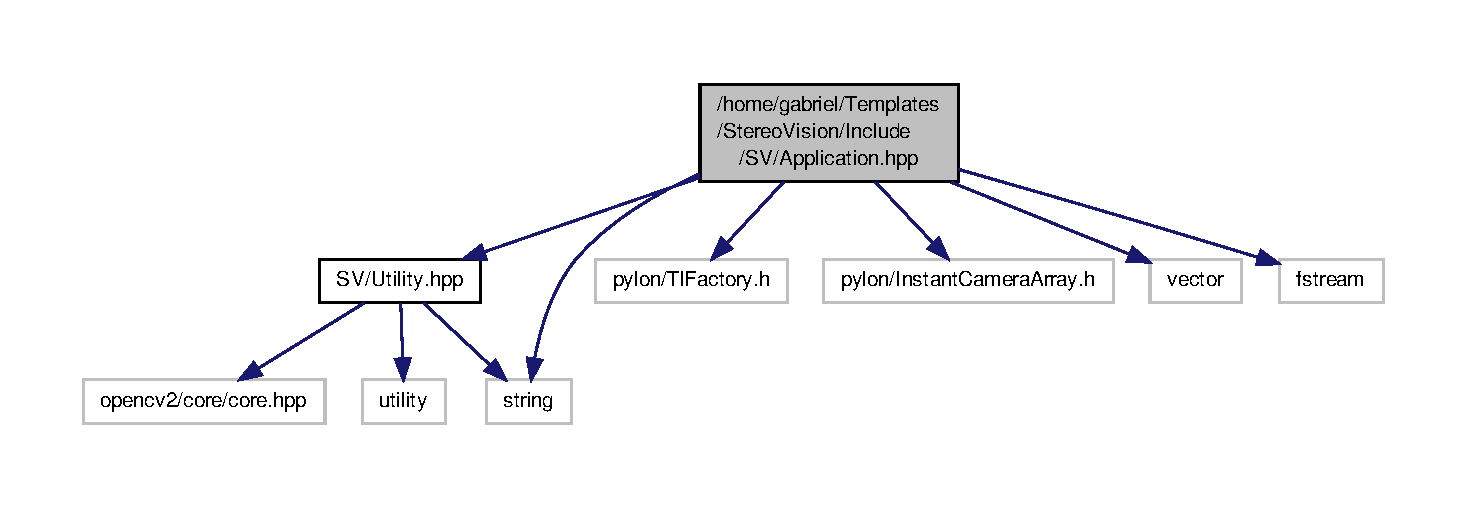
\includegraphics[width=350pt]{_application_8hpp__incl}
\end{center}
\end{figure}
This graph shows which files directly or indirectly include this file\-:
\nopagebreak
\begin{figure}[H]
\begin{center}
\leavevmode
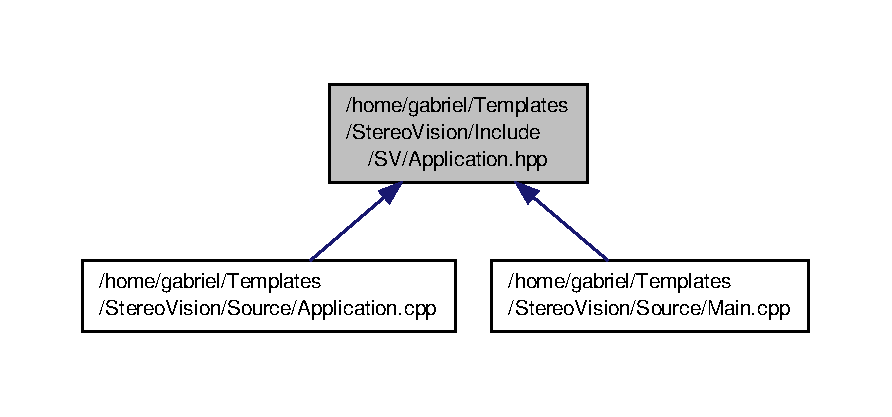
\includegraphics[width=350pt]{_application_8hpp__dep__incl}
\end{center}
\end{figure}
\subsection*{Classes}
\begin{DoxyCompactItemize}
\item 
class \hyperlink{class_application}{Application}
\end{DoxyCompactItemize}

\hypertarget{_camera_calibration_8hpp}{\section{/home/gabriel/\-Templates/\-Stereo\-Vision/\-Include/\-S\-V/\-Camera\-Calibration.hpp File Reference}
\label{_camera_calibration_8hpp}\index{/home/gabriel/\-Templates/\-Stereo\-Vision/\-Include/\-S\-V/\-Camera\-Calibration.\-hpp@{/home/gabriel/\-Templates/\-Stereo\-Vision/\-Include/\-S\-V/\-Camera\-Calibration.\-hpp}}
}
{\ttfamily \#include $<$pylon/\-Image\-Event\-Handler.\-h$>$}\\*
{\ttfamily \#include $<$opencv2/core/core.\-hpp$>$}\\*
{\ttfamily \#include $<$string$>$}\\*
{\ttfamily \#include $<$fstream$>$}\\*
Include dependency graph for Camera\-Calibration.\-hpp\-:
\nopagebreak
\begin{figure}[H]
\begin{center}
\leavevmode
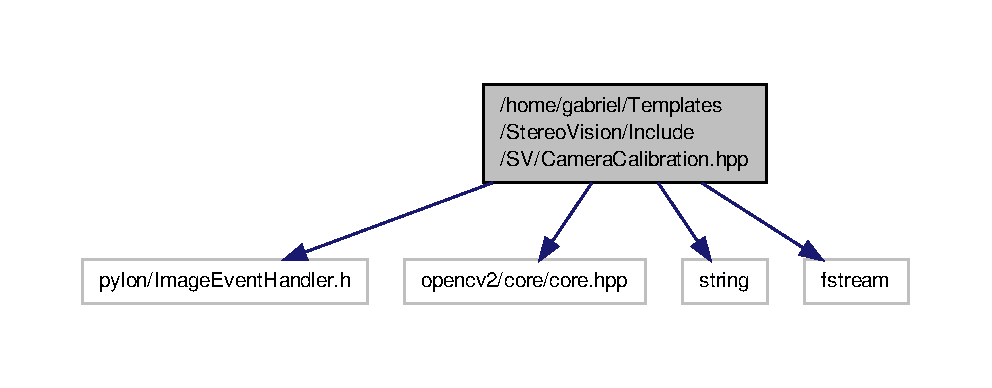
\includegraphics[width=350pt]{_camera_calibration_8hpp__incl}
\end{center}
\end{figure}
This graph shows which files directly or indirectly include this file\-:
\nopagebreak
\begin{figure}[H]
\begin{center}
\leavevmode
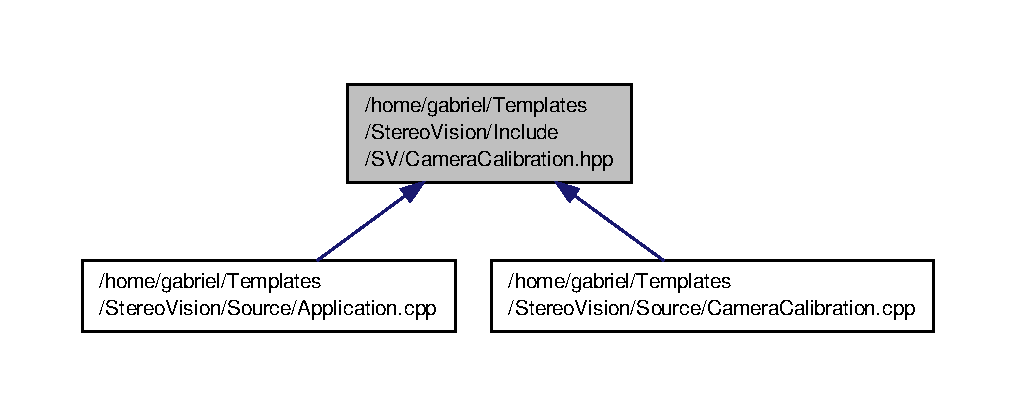
\includegraphics[width=350pt]{_camera_calibration_8hpp__dep__incl}
\end{center}
\end{figure}
\subsection*{Classes}
\begin{DoxyCompactItemize}
\item 
class \hyperlink{class_camera_calibration}{Camera\-Calibration}
\end{DoxyCompactItemize}
\subsection*{Namespaces}
\begin{DoxyCompactItemize}
\item 
\hyperlink{namespace_pylon}{Pylon}
\end{DoxyCompactItemize}
\subsection*{Constant Groups}
\begin{DoxyCompactItemize}
\item 
\hyperlink{namespace_pylon}{Pylon}
\end{DoxyCompactItemize}

\hypertarget{_camera_capture_8hpp}{\section{/home/gabriel/\-Templates/\-Stereo\-Vision/\-Include/\-S\-V/\-Camera\-Capture.hpp File Reference}
\label{_camera_capture_8hpp}\index{/home/gabriel/\-Templates/\-Stereo\-Vision/\-Include/\-S\-V/\-Camera\-Capture.\-hpp@{/home/gabriel/\-Templates/\-Stereo\-Vision/\-Include/\-S\-V/\-Camera\-Capture.\-hpp}}
}
{\ttfamily \#include $<$S\-V/\-Utility.\-hpp$>$}\\*
{\ttfamily \#include $<$pylon/\-Image\-Event\-Handler.\-h$>$}\\*
{\ttfamily \#include $<$opencv2/core/core.\-hpp$>$}\\*
{\ttfamily \#include $<$array$>$}\\*
{\ttfamily \#include $<$string$>$}\\*
Include dependency graph for Camera\-Capture.\-hpp\-:
\nopagebreak
\begin{figure}[H]
\begin{center}
\leavevmode
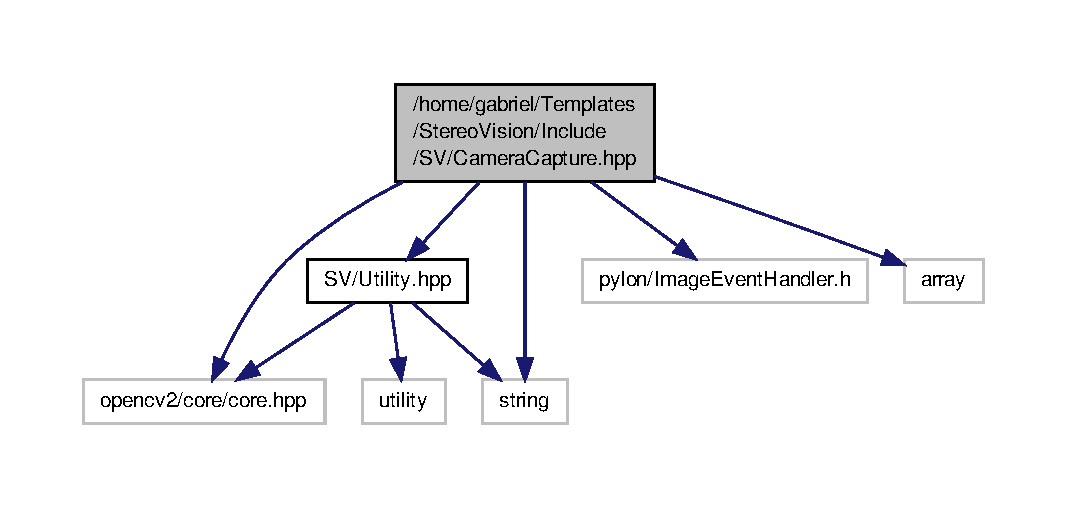
\includegraphics[width=350pt]{_camera_capture_8hpp__incl}
\end{center}
\end{figure}
This graph shows which files directly or indirectly include this file\-:
\nopagebreak
\begin{figure}[H]
\begin{center}
\leavevmode
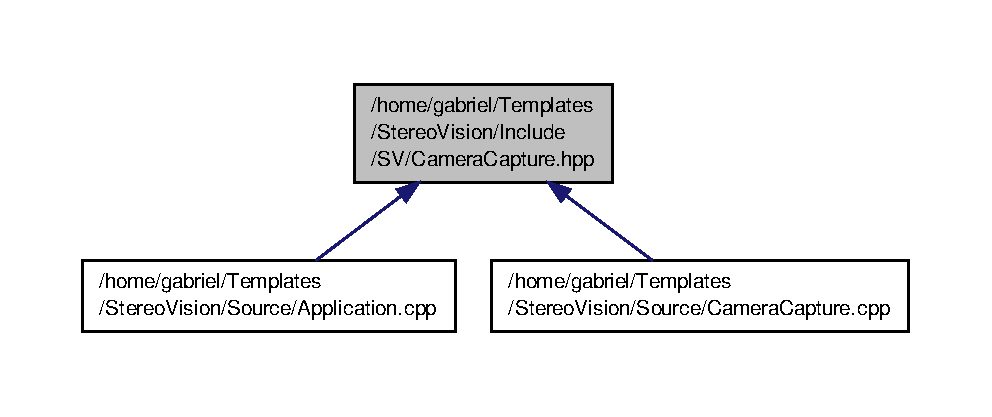
\includegraphics[width=350pt]{_camera_capture_8hpp__dep__incl}
\end{center}
\end{figure}
\subsection*{Classes}
\begin{DoxyCompactItemize}
\item 
class \hyperlink{class_camera_capture}{Camera\-Capture}
\end{DoxyCompactItemize}
\subsection*{Namespaces}
\begin{DoxyCompactItemize}
\item 
\hyperlink{namespace_pylon}{Pylon}
\end{DoxyCompactItemize}
\subsection*{Constant Groups}
\begin{DoxyCompactItemize}
\item 
\hyperlink{namespace_pylon}{Pylon}
\end{DoxyCompactItemize}

\hypertarget{_camera_configuration_8hpp}{\section{/home/gabriel/\-Templates/\-Stereo\-Vision/\-Include/\-S\-V/\-Camera\-Configuration.hpp File Reference}
\label{_camera_configuration_8hpp}\index{/home/gabriel/\-Templates/\-Stereo\-Vision/\-Include/\-S\-V/\-Camera\-Configuration.\-hpp@{/home/gabriel/\-Templates/\-Stereo\-Vision/\-Include/\-S\-V/\-Camera\-Configuration.\-hpp}}
}
{\ttfamily \#include $<$pylon/\-Configuration\-Event\-Handler.\-h$>$}\\*
{\ttfamily \#include $<$string$>$}\\*
Include dependency graph for Camera\-Configuration.\-hpp\-:
\nopagebreak
\begin{figure}[H]
\begin{center}
\leavevmode
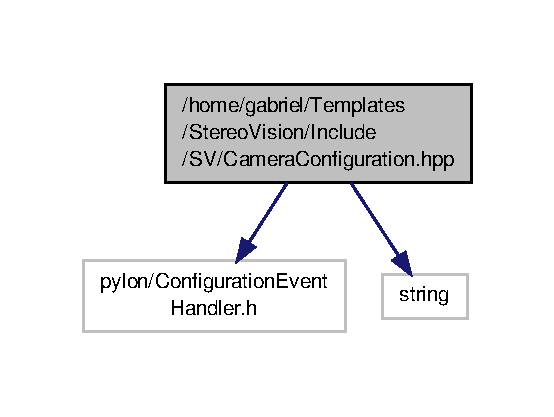
\includegraphics[width=266pt]{_camera_configuration_8hpp__incl}
\end{center}
\end{figure}
This graph shows which files directly or indirectly include this file\-:
\nopagebreak
\begin{figure}[H]
\begin{center}
\leavevmode
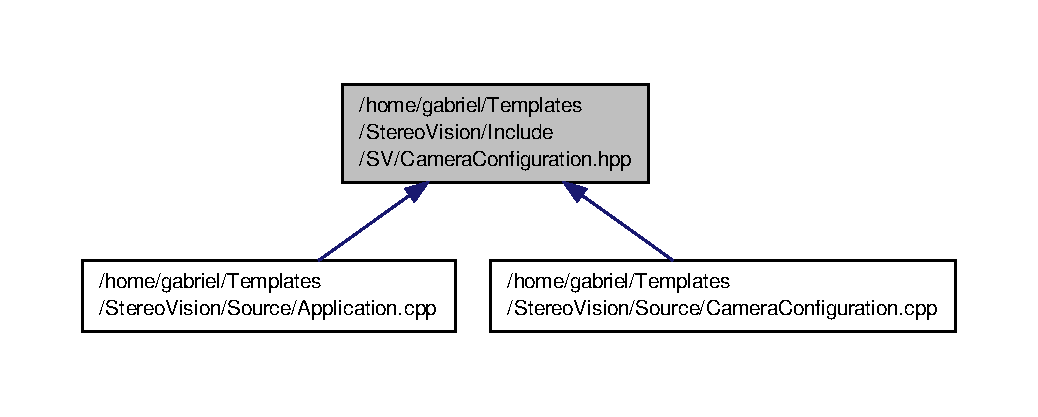
\includegraphics[width=350pt]{_camera_configuration_8hpp__dep__incl}
\end{center}
\end{figure}
\subsection*{Classes}
\begin{DoxyCompactItemize}
\item 
class \hyperlink{class_camera_configuration}{Camera\-Configuration}
\end{DoxyCompactItemize}
\subsection*{Namespaces}
\begin{DoxyCompactItemize}
\item 
\hyperlink{namespace_pylon}{Pylon}
\end{DoxyCompactItemize}
\subsection*{Constant Groups}
\begin{DoxyCompactItemize}
\item 
\hyperlink{namespace_pylon}{Pylon}
\end{DoxyCompactItemize}

\hypertarget{_utility_8hpp}{\section{/home/gabriel/\-Templates/\-Stereo\-Vision/\-Include/\-S\-V/\-Utility.hpp File Reference}
\label{_utility_8hpp}\index{/home/gabriel/\-Templates/\-Stereo\-Vision/\-Include/\-S\-V/\-Utility.\-hpp@{/home/gabriel/\-Templates/\-Stereo\-Vision/\-Include/\-S\-V/\-Utility.\-hpp}}
}
{\ttfamily \#include $<$opencv2/core/core.\-hpp$>$}\\*
{\ttfamily \#include $<$string$>$}\\*
{\ttfamily \#include $<$utility$>$}\\*
Include dependency graph for Utility.\-hpp\-:
\nopagebreak
\begin{figure}[H]
\begin{center}
\leavevmode
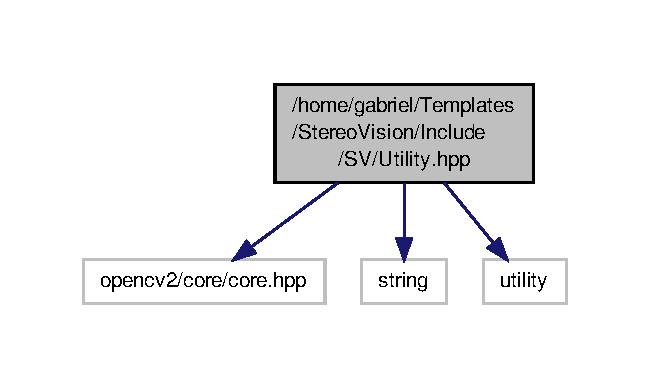
\includegraphics[width=312pt]{_utility_8hpp__incl}
\end{center}
\end{figure}
This graph shows which files directly or indirectly include this file\-:
\nopagebreak
\begin{figure}[H]
\begin{center}
\leavevmode
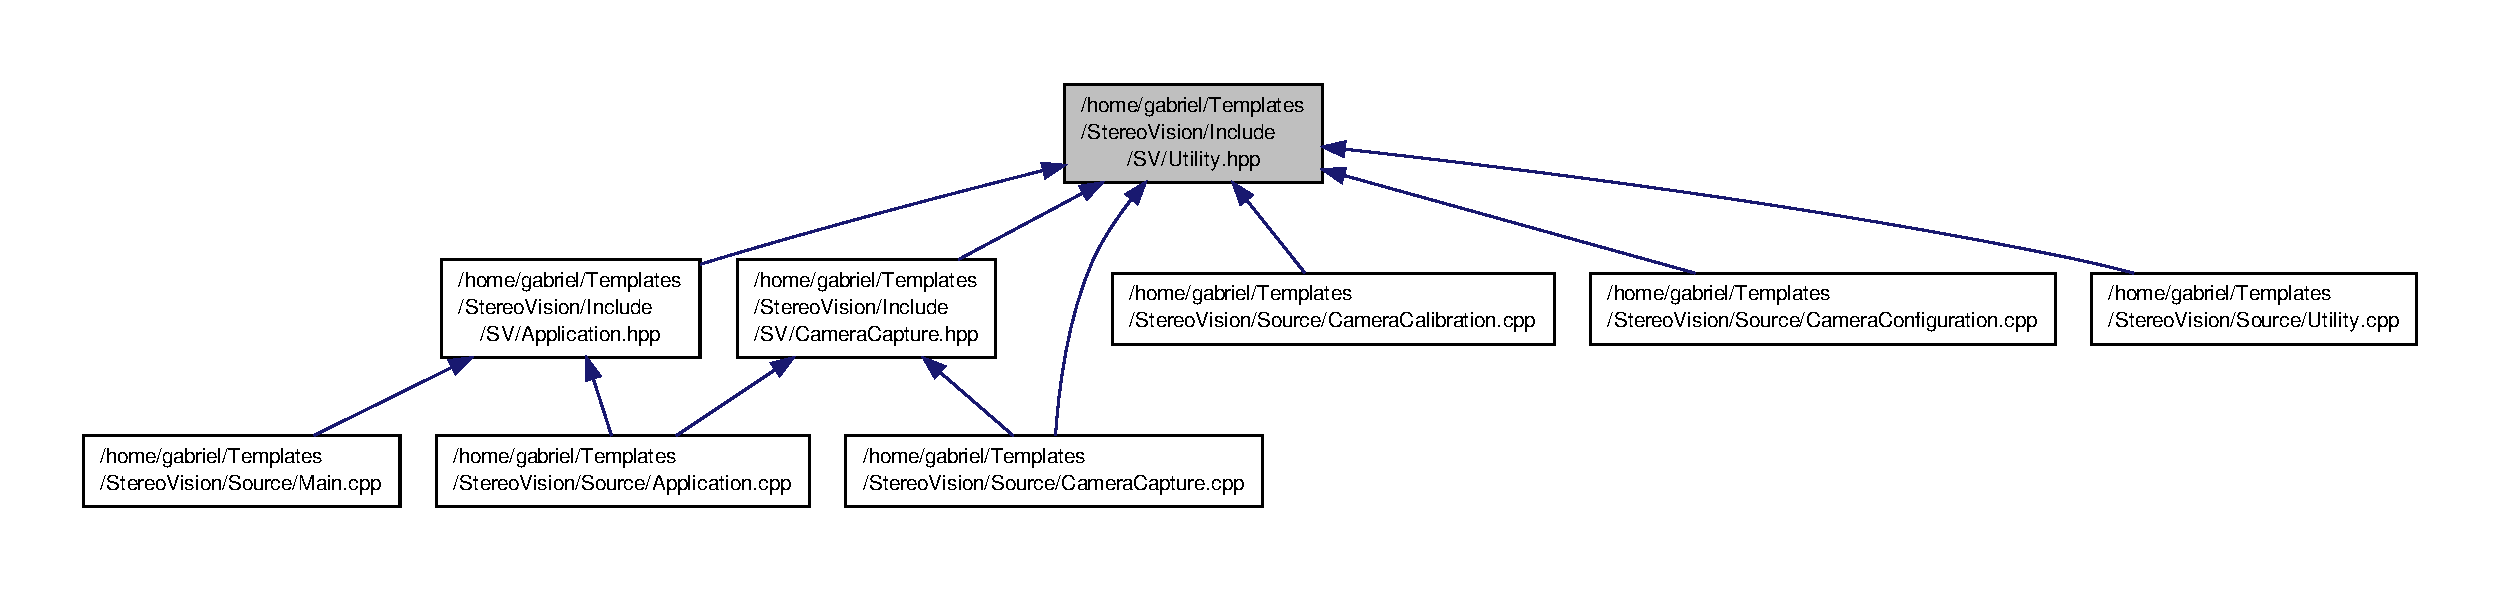
\includegraphics[width=350pt]{_utility_8hpp__dep__incl}
\end{center}
\end{figure}
\subsection*{Classes}
\begin{DoxyCompactItemize}
\item 
struct \hyperlink{struct_s_v_1_1_calibration_pattern}{S\-V\-::\-Calibration\-Pattern}
\item 
struct \hyperlink{struct_s_v_1_1_stereo_photo}{S\-V\-::\-Stereo\-Photo}
\end{DoxyCompactItemize}
\subsection*{Namespaces}
\begin{DoxyCompactItemize}
\item 
\hyperlink{namespace_s_v}{S\-V}
\end{DoxyCompactItemize}
\subsection*{Constant Groups}
\begin{DoxyCompactItemize}
\item 
\hyperlink{namespace_s_v}{S\-V}
\end{DoxyCompactItemize}
\subsection*{Functions}
\begin{DoxyCompactItemize}
\item 
std\-::string \hyperlink{namespace_s_v_a9f7b63fd7ff59d018c9033a412abc4c0}{S\-V\-::get\-Timestamp} ()
\item 
std\-::string \hyperlink{namespace_s_v_ae32886e460af95f632f666beb6846946}{S\-V\-::load\-Calibration\-Timestamp\-File} ()
\item 
void \hyperlink{namespace_s_v_a290f15aeacbb1347daab1947fd4f25a4}{S\-V\-::save\-Calibration\-Timestamp\-File} ()
\item 
Calibration\-Pattern \hyperlink{namespace_s_v_a2eeee0cf678d9d481d3d3549b151a4a6}{S\-V\-::load\-Calibration\-Pattern\-File} ()
\item 
void \hyperlink{namespace_s_v_ae0b57b979ffff6071335b0e3af71d010}{S\-V\-::save\-Calibration\-Pattern\-File} (unsigned int w, unsigned int h, float s)
\item 
int \hyperlink{namespace_s_v_aac43c382d355779c28aac79e5f1a1f2f}{S\-V\-::fork\-Exec\-Stereo\-Calibration\-Module} (unsigned int w, unsigned int h, float s)
\item 
cv\-::\-Scalar \hyperlink{namespace_s_v_ad372136d1d33214cd8b7baa169fca11c}{S\-V\-::open\-C\-V\-Random\-Color} (cv\-::\-R\-N\-G \&rng)
\end{DoxyCompactItemize}
\subsection*{Variables}
\begin{DoxyCompactItemize}
\item 
const int \hyperlink{namespace_s_v_aa2acf99b8a3b122f688769ef693c30ae}{S\-V\-::\-M\-A\-X\-\_\-\-N\-U\-M\-B\-E\-R\-\_\-\-O\-F\-\_\-\-C\-A\-M\-E\-R\-A\-S} = 2
\item 
const char $\ast$ \hyperlink{namespace_s_v_aa00fc841744191453046361becae6ae6}{S\-V\-::\-C\-O\-N\-F\-I\-G\-U\-R\-A\-T\-I\-O\-N\-\_\-\-F\-I\-L\-E} = \char`\"{}Config/Camera/default\-\_\-linux.\-pfs\char`\"{}
\item 
int \hyperlink{namespace_s_v_a778a8d19ba21816aca4e8ca6c2dcd4a2}{S\-V\-::\-M\-A\-I\-N\-\_\-\-L\-O\-O\-P\-\_\-\-I\-T\-E\-R\-A\-T\-I\-O\-N\-\_\-\-T\-I\-M\-E} = 0
\item 
const int \hyperlink{namespace_s_v_aa245d3d1f71d5a419cefdc42626b1c07}{S\-V\-::\-I\-N\-T\-E\-R\-\_\-\-P\-A\-C\-K\-E\-T\-\_\-\-D\-E\-L\-A\-Y} = 8192
\item 
const int \hyperlink{namespace_s_v_a91d9ea38d5f6a4803e3e94ad8c9a722a}{S\-V\-::\-F\-R\-A\-M\-E\-\_\-\-T\-R\-A\-N\-S\-M\-I\-S\-S\-I\-O\-N\-\_\-\-D\-E\-L\-A\-Y} = 4096 + \hyperlink{namespace_s_v_a778a8d19ba21816aca4e8ca6c2dcd4a2}{S\-V\-::\-M\-A\-I\-N\-\_\-\-L\-O\-O\-P\-\_\-\-I\-T\-E\-R\-A\-T\-I\-O\-N\-\_\-\-T\-I\-M\-E}
\item 
const std\-::string \hyperlink{namespace_s_v_a07b166ccd37fa68ea084cebb48a1f6f7}{S\-V\-::\-C\-A\-L\-I\-B\-R\-A\-T\-I\-O\-N\-\_\-\-B\-I\-N} = \char`\"{}Stereo\-Calibration\char`\"{}
\item 
const std\-::string \hyperlink{namespace_s_v_a25683376004000d485cf2c87db0f6b2a}{S\-V\-::\-C\-A\-L\-I\-B\-R\-A\-T\-I\-O\-N\-\_\-\-T\-I\-M\-E\-S\-T\-A\-M\-P\-\_\-\-F\-I\-L\-E} = \char`\"{}Config/Calibration/timestamp.\-txt\char`\"{}
\item 
const std\-::string \hyperlink{namespace_s_v_ab14088c3b114b4905a5064056e160576}{S\-V\-::\-C\-A\-L\-I\-B\-R\-A\-T\-I\-O\-N\-\_\-\-P\-A\-T\-T\-E\-R\-N\-\_\-\-F\-I\-L\-E} = \char`\"{}Config/Calibration/pattern.\-txt\char`\"{}
\item 
const std\-::string \hyperlink{namespace_s_v_a08efa5f4f7f6a650b132fe6ce146c7a6}{S\-V\-::\-C\-A\-L\-I\-B\-R\-A\-T\-I\-O\-N\-\_\-\-X\-M\-L\-\_\-\-F\-I\-L\-E\-S\-\_\-\-P\-A\-T\-H} = \char`\"{}Config/Calibration/X\-M\-L\-Files/\char`\"{}
\item 
const std\-::string \hyperlink{namespace_s_v_a31f33ecf5d55099dbdcbf01cbdc8f85e}{S\-V\-::\-C\-A\-L\-I\-B\-R\-A\-T\-I\-O\-N\-\_\-\-I\-M\-A\-G\-E\-S\-\_\-\-F\-I\-L\-E} = \char`\"{}Config/Calibration/list.\-txt\char`\"{}
\item 
const std\-::string \hyperlink{namespace_s_v_aca9f280a6ae4110ddbfcb3db20c40931}{S\-V\-::\-C\-A\-L\-I\-B\-R\-A\-T\-I\-O\-N\-\_\-\-I\-M\-A\-G\-E\-S\-\_\-\-P\-A\-T\-H} = \char`\"{}Config/Calibration/Images/\char`\"{}
\item 
const std\-::string \hyperlink{namespace_s_v_a7eee3c30084ee151a5d8e793f448dfca}{S\-V\-::\-C\-A\-L\-I\-B\-R\-A\-T\-I\-O\-N\-\_\-\-I\-M\-A\-G\-E\-\_\-\-L\-E\-F\-T} = \char`\"{}left.\-ppm\char`\"{}
\item 
const std\-::string \hyperlink{namespace_s_v_a6b93f40cb116005baad0fa89d5e3ded3}{S\-V\-::\-C\-A\-L\-I\-B\-R\-A\-T\-I\-O\-N\-\_\-\-I\-M\-A\-G\-E\-\_\-\-R\-I\-G\-H\-T} = \char`\"{}right.\-ppm\char`\"{}
\item 
const std\-::string \hyperlink{namespace_s_v_af29adc97546d0aacc73089470104b7e6}{S\-V\-::\-N\-O\-T\-\_\-\-C\-A\-L\-I\-B\-R\-A\-T\-E\-D} = \char`\"{}N\-O\-T\-\_\-\-C\-A\-L\-I\-B\-R\-A\-T\-E\-D\char`\"{}
\item 
bool \hyperlink{namespace_s_v_abef27351d2e2c8b13783f080571edca8}{S\-V\-::\-E\-M\-U\-L\-A\-T\-I\-O\-N\-\_\-\-M\-O\-D\-E} = false
\item 
const std\-::string \hyperlink{namespace_s_v_ab43026f6f6ee1b8e5cc36194a2ea9e6b}{S\-V\-::\-E\-M\-U\-L\-A\-T\-E\-D\-\_\-\-C\-A\-M\-E\-R\-A} = \char`\"{}Emulation\char`\"{}
\item 
const std\-::string \hyperlink{namespace_s_v_a4a601cd489e8ca00c55bb2785c8bb5d9}{S\-V\-::\-E\-M\-U\-L\-A\-T\-E\-D\-\_\-\-I\-M\-A\-G\-E\-S\-\_\-\-F\-I\-L\-E} = \char`\"{}Config/Calibration/list\-\_\-emulation.\-txt\char`\"{}
\item 
const std\-::string \hyperlink{namespace_s_v_ab98fb68d38e7637f92d456f945dfd2ff}{S\-V\-::\-E\-M\-U\-L\-A\-T\-E\-D\-\_\-\-I\-M\-A\-G\-E\-S\-\_\-\-P\-A\-T\-H} = \hyperlink{namespace_s_v_aca9f280a6ae4110ddbfcb3db20c40931}{S\-V\-::\-C\-A\-L\-I\-B\-R\-A\-T\-I\-O\-N\-\_\-\-I\-M\-A\-G\-E\-S\-\_\-\-P\-A\-T\-H} + \char`\"{}Emulation/\char`\"{}
\item 
const std\-::string \hyperlink{namespace_s_v_aa04b6739e3012b22c033d003c26d5584}{S\-V\-::line\-Break} = \char`\"{}================================\textbackslash{}n\char`\"{}
\end{DoxyCompactItemize}

\hypertarget{_stereo_calibration_8cpp}{\section{/home/gabriel/\-Templates/\-Stereo\-Vision/\-Modules/\-Stereo\-Calibration/\-Stereo\-Calibration.cpp File Reference}
\label{_stereo_calibration_8cpp}\index{/home/gabriel/\-Templates/\-Stereo\-Vision/\-Modules/\-Stereo\-Calibration/\-Stereo\-Calibration.\-cpp@{/home/gabriel/\-Templates/\-Stereo\-Vision/\-Modules/\-Stereo\-Calibration/\-Stereo\-Calibration.\-cpp}}
}
{\ttfamily \#include \char`\"{}cv.\-h\char`\"{}}\\*
{\ttfamily \#include \char`\"{}cxmisc.\-h\char`\"{}}\\*
{\ttfamily \#include \char`\"{}highgui.\-h\char`\"{}}\\*
{\ttfamily \#include \char`\"{}cvaux.\-h\char`\"{}}\\*
{\ttfamily \#include $<$vector$>$}\\*
{\ttfamily \#include $<$string$>$}\\*
{\ttfamily \#include $<$algorithm$>$}\\*
{\ttfamily \#include $<$stdio.\-h$>$}\\*
{\ttfamily \#include $<$stdlib.\-h$>$}\\*
{\ttfamily \#include $<$ctype.\-h$>$}\\*
Include dependency graph for Stereo\-Calibration.\-cpp\-:
\nopagebreak
\begin{figure}[H]
\begin{center}
\leavevmode
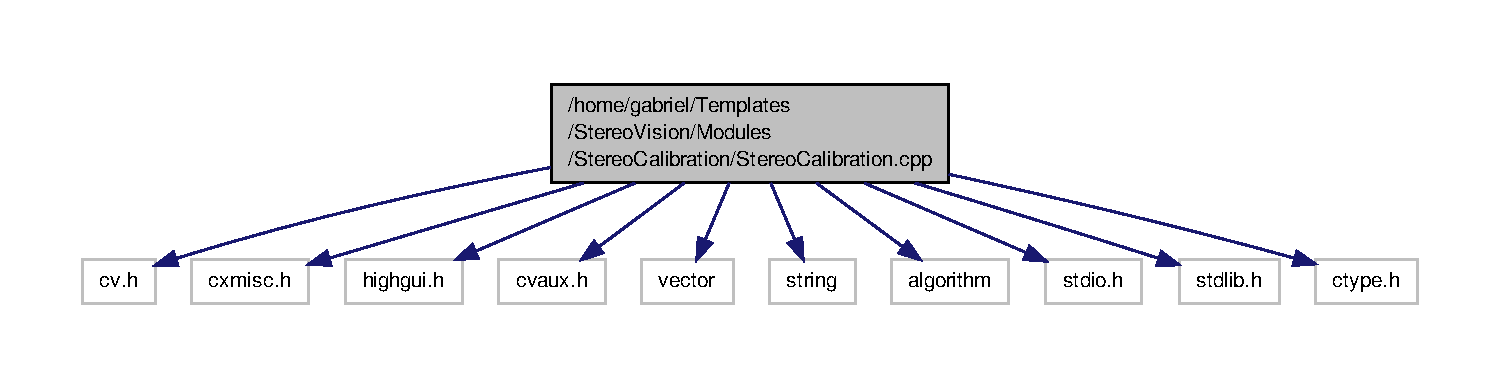
\includegraphics[width=350pt]{_stereo_calibration_8cpp__incl}
\end{center}
\end{figure}
\subsection*{Functions}
\begin{DoxyCompactItemize}
\item 
int \hyperlink{_stereo_calibration_8cpp_a0ddf1224851353fc92bfbff6f499fa97}{main} (int argc, char $\ast$argv\mbox{[}$\,$\mbox{]})
\end{DoxyCompactItemize}


\subsection{Function Documentation}
\hypertarget{_stereo_calibration_8cpp_a0ddf1224851353fc92bfbff6f499fa97}{\index{Stereo\-Calibration.\-cpp@{Stereo\-Calibration.\-cpp}!main@{main}}
\index{main@{main}!StereoCalibration.cpp@{Stereo\-Calibration.\-cpp}}
\subsubsection[{main}]{\setlength{\rightskip}{0pt plus 5cm}int main (
\begin{DoxyParamCaption}
\item[{int}]{argc, }
\item[{char $\ast$}]{argv\mbox{[}$\,$\mbox{]}}
\end{DoxyParamCaption}
)}}\label{_stereo_calibration_8cpp_a0ddf1224851353fc92bfbff6f499fa97}


Definition at line 463 of file Stereo\-Calibration.\-cpp.


\hypertarget{_r_e_a_d_m_e_8md}{\section{/home/gabriel/\-Templates/\-Stereo\-Vision/\-R\-E\-A\-D\-M\-E.md File Reference}
\label{_r_e_a_d_m_e_8md}\index{/home/gabriel/\-Templates/\-Stereo\-Vision/\-R\-E\-A\-D\-M\-E.\-md@{/home/gabriel/\-Templates/\-Stereo\-Vision/\-R\-E\-A\-D\-M\-E.\-md}}
}

\hypertarget{_application_8cpp}{\section{/home/gabriel/\-Templates/\-Stereo\-Vision/\-Source/\-Application.cpp File Reference}
\label{_application_8cpp}\index{/home/gabriel/\-Templates/\-Stereo\-Vision/\-Source/\-Application.\-cpp@{/home/gabriel/\-Templates/\-Stereo\-Vision/\-Source/\-Application.\-cpp}}
}
{\ttfamily \#include $<$S\-V/\-Application.\-hpp$>$}\\*
{\ttfamily \#include $<$S\-V/\-Camera\-Calibration.\-hpp$>$}\\*
{\ttfamily \#include $<$S\-V/\-Camera\-Capture.\-hpp$>$}\\*
{\ttfamily \#include $<$S\-V/\-Camera\-Configuration.\-hpp$>$}\\*
{\ttfamily \#include $<$opencv2/highgui/highgui.\-hpp$>$}\\*
{\ttfamily \#include $<$memory$>$}\\*
{\ttfamily \#include $<$cassert$>$}\\*
{\ttfamily \#include $<$iostream$>$}\\*
{\ttfamily \#include $<$stdexcept$>$}\\*
Include dependency graph for Application.\-cpp\-:
\nopagebreak
\begin{figure}[H]
\begin{center}
\leavevmode
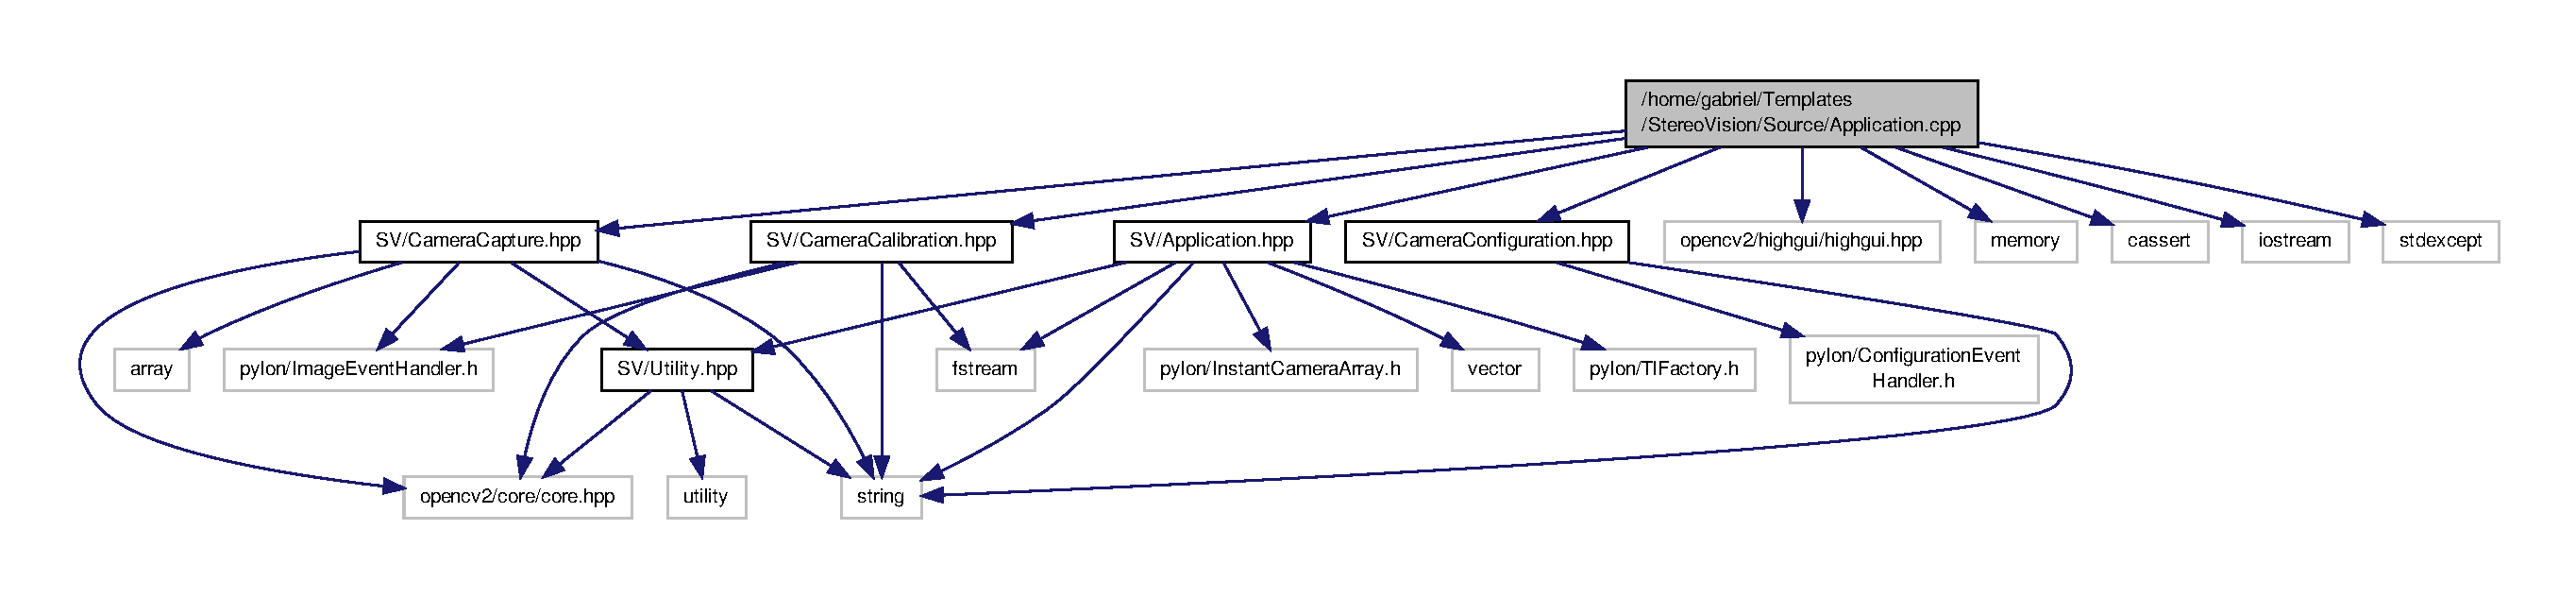
\includegraphics[width=350pt]{_application_8cpp__incl}
\end{center}
\end{figure}

\hypertarget{_camera_calibration_8cpp}{\section{/home/gabriel/\-Templates/\-Stereo\-Vision/\-Source/\-Camera\-Calibration.cpp File Reference}
\label{_camera_calibration_8cpp}\index{/home/gabriel/\-Templates/\-Stereo\-Vision/\-Source/\-Camera\-Calibration.\-cpp@{/home/gabriel/\-Templates/\-Stereo\-Vision/\-Source/\-Camera\-Calibration.\-cpp}}
}
{\ttfamily \#include $<$S\-V/\-Camera\-Calibration.\-hpp$>$}\\*
{\ttfamily \#include $<$S\-V/\-Utility.\-hpp$>$}\\*
{\ttfamily \#include $<$pylon/\-Instant\-Camera.\-h$>$}\\*
{\ttfamily \#include $<$pylon/\-Grab\-Result\-Ptr.\-h$>$}\\*
{\ttfamily \#include $<$opencv2/highgui/highgui.\-hpp$>$}\\*
{\ttfamily \#include $<$opencv2/imgproc/imgproc.\-hpp$>$}\\*
{\ttfamily \#include $<$opencv2/calib3d/calib3d.\-hpp$>$}\\*
{\ttfamily \#include $<$iostream$>$}\\*
{\ttfamily \#include $<$fstream$>$}\\*
Include dependency graph for Camera\-Calibration.\-cpp\-:
\nopagebreak
\begin{figure}[H]
\begin{center}
\leavevmode
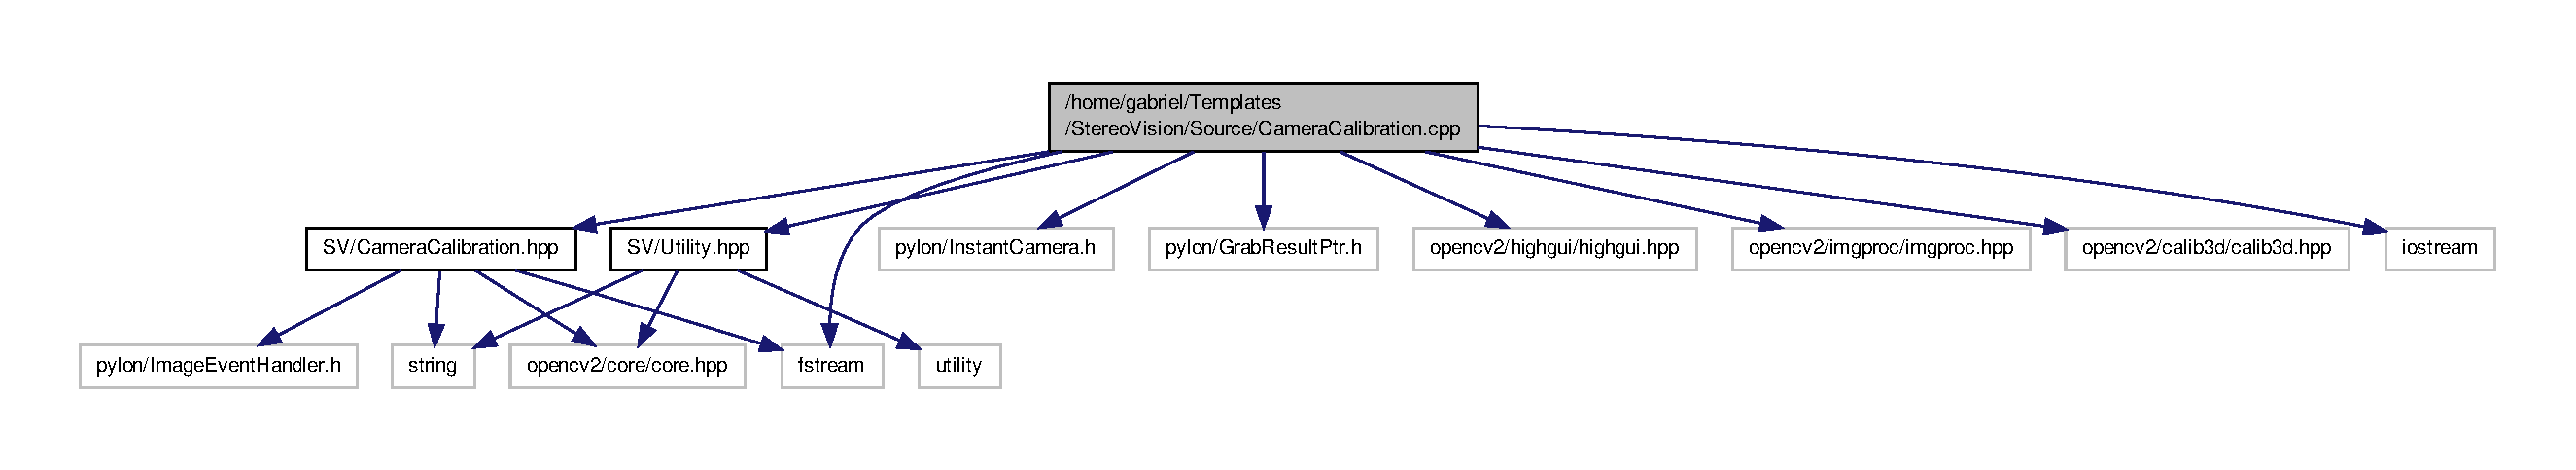
\includegraphics[width=350pt]{_camera_calibration_8cpp__incl}
\end{center}
\end{figure}

\hypertarget{_camera_capture_8cpp}{\section{/home/gabriel/\-Templates/\-Stereo\-Vision/\-Source/\-Camera\-Capture.cpp File Reference}
\label{_camera_capture_8cpp}\index{/home/gabriel/\-Templates/\-Stereo\-Vision/\-Source/\-Camera\-Capture.\-cpp@{/home/gabriel/\-Templates/\-Stereo\-Vision/\-Source/\-Camera\-Capture.\-cpp}}
}
{\ttfamily \#include $<$S\-V/\-Camera\-Capture.\-hpp$>$}\\*
{\ttfamily \#include $<$S\-V/\-Utility.\-hpp$>$}\\*
{\ttfamily \#include $<$pylon/\-Instant\-Camera.\-h$>$}\\*
{\ttfamily \#include $<$pylon/\-Grab\-Result\-Ptr.\-h$>$}\\*
{\ttfamily \#include $<$opencv2/highgui/highgui.\-hpp$>$}\\*
{\ttfamily \#include $<$opencv2/imgproc/imgproc.\-hpp$>$}\\*
{\ttfamily \#include $<$opencv2/calib3d/calib3d.\-hpp$>$}\\*
{\ttfamily \#include $<$iostream$>$}\\*
Include dependency graph for Camera\-Capture.\-cpp\-:
\nopagebreak
\begin{figure}[H]
\begin{center}
\leavevmode
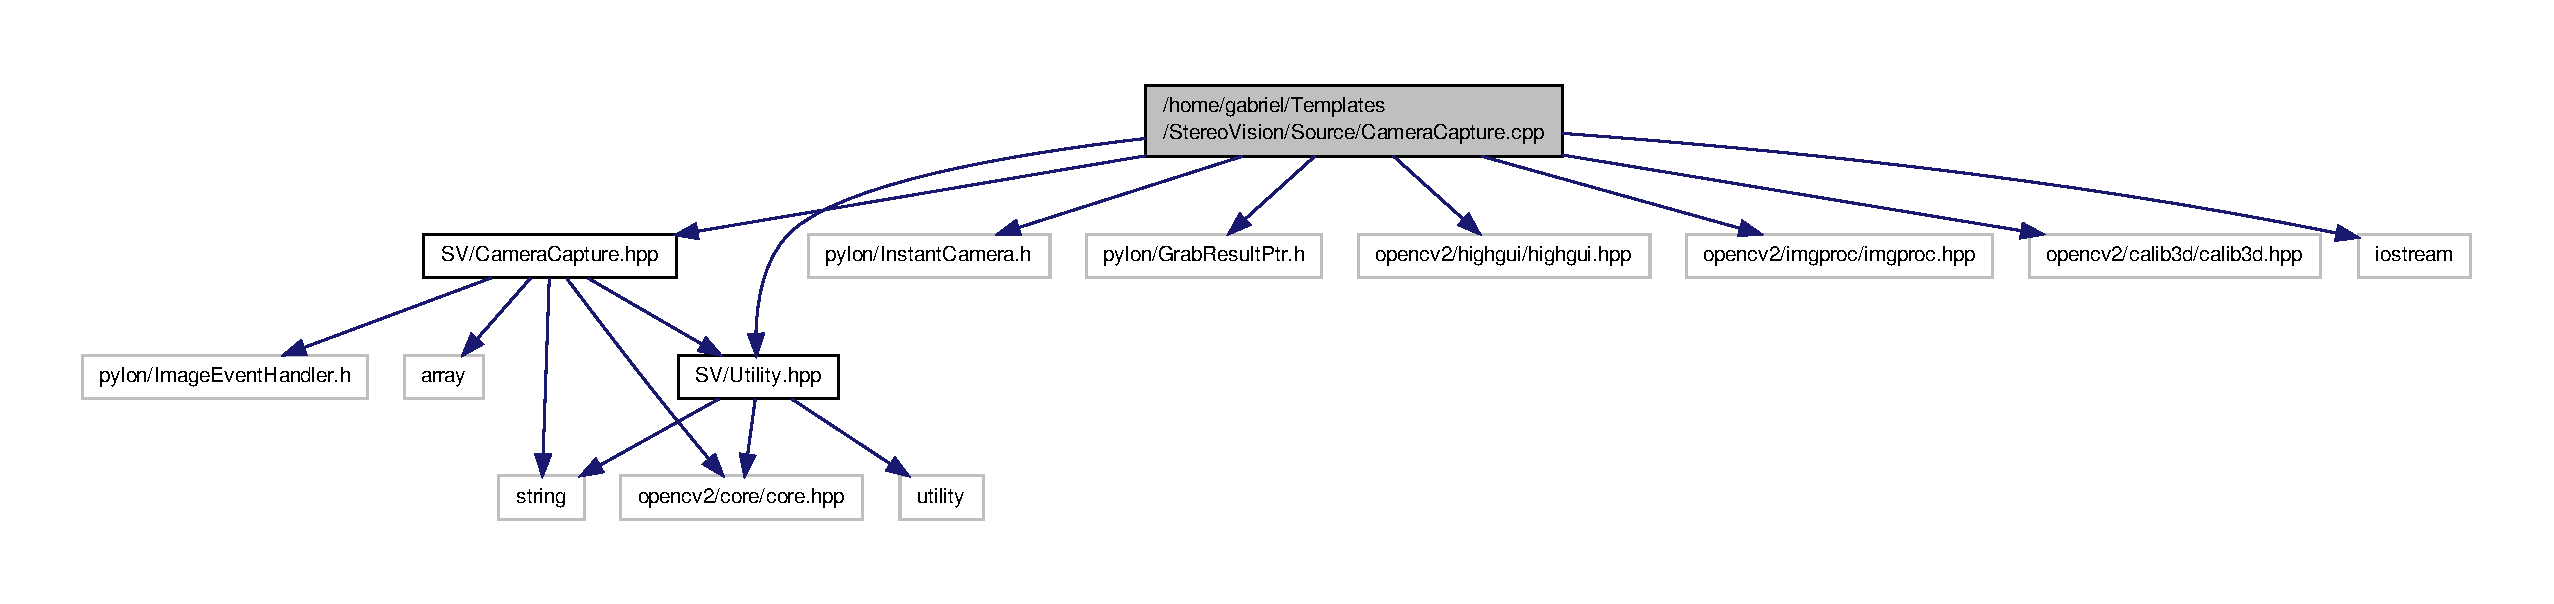
\includegraphics[width=350pt]{_camera_capture_8cpp__incl}
\end{center}
\end{figure}
\subsection*{Functions}
\begin{DoxyCompactItemize}
\item 
\hyperlink{_camera_capture_8cpp_a402ec501906aa2268892e021e54dbd11}{m\-Calibration\-Matrices\-Names} (\{\char`\"{}Q\char`\"{},\char`\"{}mx1\char`\"{},\char`\"{}my1\char`\"{},\char`\"{}mx2\char`\"{},\char`\"{}my2\char`\"{}\})
\item 
\hyperlink{_camera_capture_8cpp_a0dcdf9c5f3116470f6dfcb64fd5e1799}{m\-Pattern\-Size} ()
\item 
\hyperlink{_camera_capture_8cpp_a26b9b87dc68679ffef91a4e4f68b4bb9}{m\-Stereo\-Photo\-Ptr} (stereo\-Photo\-Ptr)
\end{DoxyCompactItemize}


\subsection{Function Documentation}
\hypertarget{_camera_capture_8cpp_a402ec501906aa2268892e021e54dbd11}{\index{Camera\-Capture.\-cpp@{Camera\-Capture.\-cpp}!m\-Calibration\-Matrices\-Names@{m\-Calibration\-Matrices\-Names}}
\index{m\-Calibration\-Matrices\-Names@{m\-Calibration\-Matrices\-Names}!CameraCapture.cpp@{Camera\-Capture.\-cpp}}
\subsubsection[{m\-Calibration\-Matrices\-Names}]{\setlength{\rightskip}{0pt plus 5cm}m\-Calibration\-Matrices\-Names (
\begin{DoxyParamCaption}
\item[{\{\char`\"{}Q\char`\"{},\char`\"{}mx1\char`\"{},\char`\"{}my1\char`\"{},\char`\"{}mx2\char`\"{},\char`\"{}my2\char`\"{}\}}]{}
\end{DoxyParamCaption}
)}}\label{_camera_capture_8cpp_a402ec501906aa2268892e021e54dbd11}


Here is the caller graph for this function\-:
\nopagebreak
\begin{figure}[H]
\begin{center}
\leavevmode
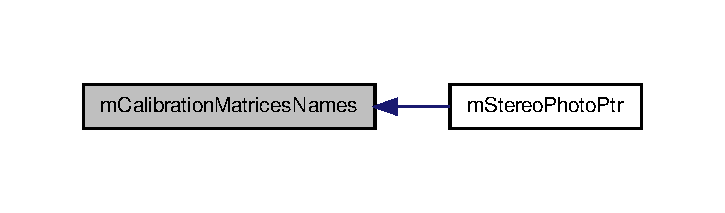
\includegraphics[width=348pt]{_camera_capture_8cpp_a402ec501906aa2268892e021e54dbd11_icgraph}
\end{center}
\end{figure}


\hypertarget{_camera_capture_8cpp_a0dcdf9c5f3116470f6dfcb64fd5e1799}{\index{Camera\-Capture.\-cpp@{Camera\-Capture.\-cpp}!m\-Pattern\-Size@{m\-Pattern\-Size}}
\index{m\-Pattern\-Size@{m\-Pattern\-Size}!CameraCapture.cpp@{Camera\-Capture.\-cpp}}
\subsubsection[{m\-Pattern\-Size}]{\setlength{\rightskip}{0pt plus 5cm}m\-Pattern\-Size (
\begin{DoxyParamCaption}
{}
\end{DoxyParamCaption}
)}}\label{_camera_capture_8cpp_a0dcdf9c5f3116470f6dfcb64fd5e1799}


Here is the caller graph for this function\-:
\nopagebreak
\begin{figure}[H]
\begin{center}
\leavevmode
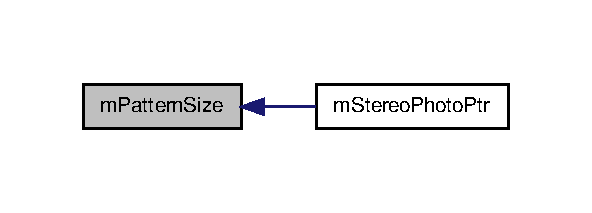
\includegraphics[width=284pt]{_camera_capture_8cpp_a0dcdf9c5f3116470f6dfcb64fd5e1799_icgraph}
\end{center}
\end{figure}


\hypertarget{_camera_capture_8cpp_a26b9b87dc68679ffef91a4e4f68b4bb9}{\index{Camera\-Capture.\-cpp@{Camera\-Capture.\-cpp}!m\-Stereo\-Photo\-Ptr@{m\-Stereo\-Photo\-Ptr}}
\index{m\-Stereo\-Photo\-Ptr@{m\-Stereo\-Photo\-Ptr}!CameraCapture.cpp@{Camera\-Capture.\-cpp}}
\subsubsection[{m\-Stereo\-Photo\-Ptr}]{\setlength{\rightskip}{0pt plus 5cm}m\-Stereo\-Photo\-Ptr (
\begin{DoxyParamCaption}
\item[{stereo\-Photo\-Ptr}]{}
\end{DoxyParamCaption}
)}}\label{_camera_capture_8cpp_a26b9b87dc68679ffef91a4e4f68b4bb9}


Definition at line 26 of file Camera\-Capture.\-cpp.



Here is the call graph for this function\-:
\nopagebreak
\begin{figure}[H]
\begin{center}
\leavevmode
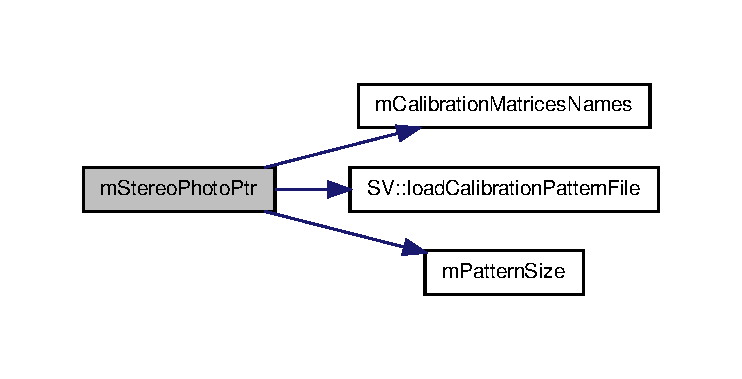
\includegraphics[width=350pt]{_camera_capture_8cpp_a26b9b87dc68679ffef91a4e4f68b4bb9_cgraph}
\end{center}
\end{figure}



\hypertarget{_camera_configuration_8cpp}{\section{/home/gabriel/\-Templates/\-Stereo\-Vision/\-Source/\-Camera\-Configuration.cpp File Reference}
\label{_camera_configuration_8cpp}\index{/home/gabriel/\-Templates/\-Stereo\-Vision/\-Source/\-Camera\-Configuration.\-cpp@{/home/gabriel/\-Templates/\-Stereo\-Vision/\-Source/\-Camera\-Configuration.\-cpp}}
}
{\ttfamily \#include $<$S\-V/\-Camera\-Configuration.\-hpp$>$}\\*
{\ttfamily \#include $<$S\-V/\-Utility.\-hpp$>$}\\*
{\ttfamily \#include $<$pylon/\-Instant\-Camera.\-h$>$}\\*
{\ttfamily \#include $<$pylon/\-Feature\-Persistence.\-h$>$}\\*
{\ttfamily \#include $<$Gen\-Api/\-I\-Node\-Map.\-h$>$}\\*
{\ttfamily \#include $<$Gen\-Api/\-Types.\-h$>$}\\*
{\ttfamily \#include $<$iostream$>$}\\*
Include dependency graph for Camera\-Configuration.\-cpp\-:
\nopagebreak
\begin{figure}[H]
\begin{center}
\leavevmode
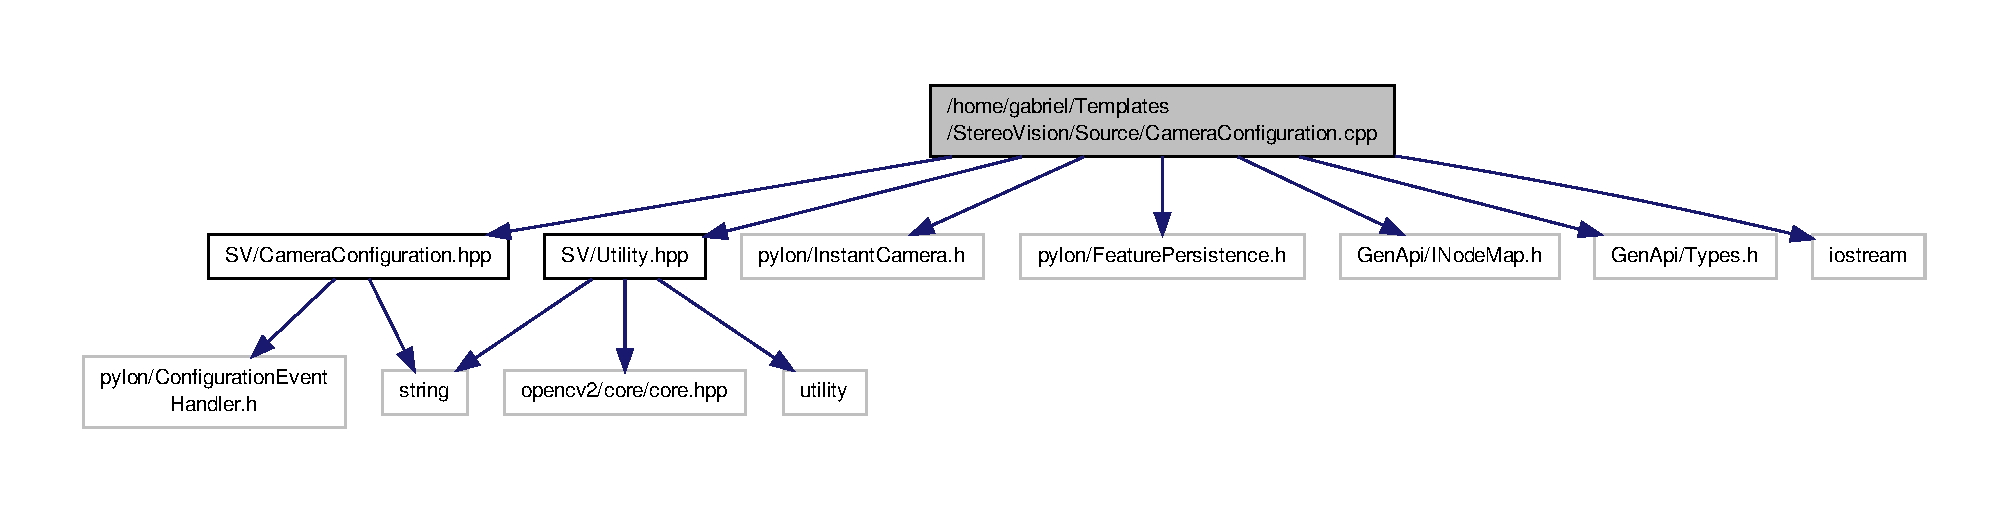
\includegraphics[width=350pt]{_camera_configuration_8cpp__incl}
\end{center}
\end{figure}

\hypertarget{_main_8cpp}{\section{/home/gabriel/\-Templates/\-Stereo\-Vision/\-Source/\-Main.cpp File Reference}
\label{_main_8cpp}\index{/home/gabriel/\-Templates/\-Stereo\-Vision/\-Source/\-Main.\-cpp@{/home/gabriel/\-Templates/\-Stereo\-Vision/\-Source/\-Main.\-cpp}}
}
{\ttfamily \#include $<$S\-V/\-Application.\-hpp$>$}\\*
{\ttfamily \#include $<$stdexcept$>$}\\*
{\ttfamily \#include $<$iostream$>$}\\*
Include dependency graph for Main.\-cpp\-:
\nopagebreak
\begin{figure}[H]
\begin{center}
\leavevmode
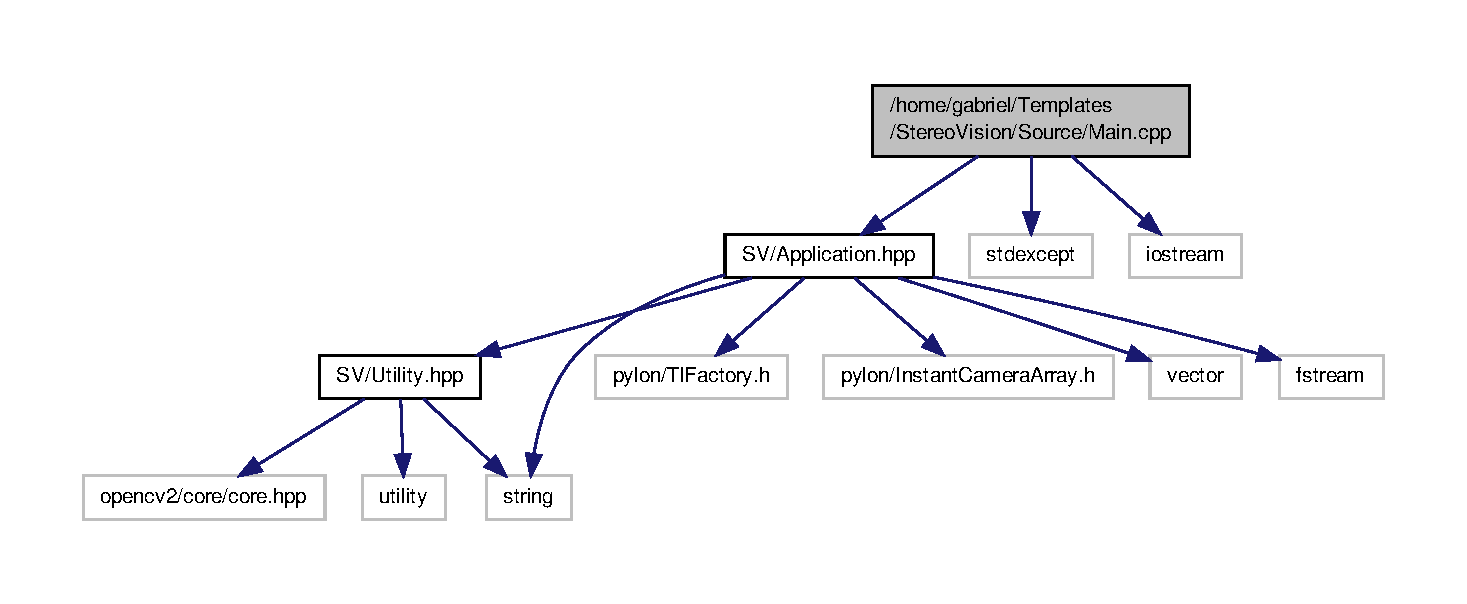
\includegraphics[width=350pt]{_main_8cpp__incl}
\end{center}
\end{figure}
\subsection*{Functions}
\begin{DoxyCompactItemize}
\item 
int \hyperlink{_main_8cpp_ae66f6b31b5ad750f1fe042a706a4e3d4}{main} ()
\end{DoxyCompactItemize}


\subsection{Function Documentation}
\hypertarget{_main_8cpp_ae66f6b31b5ad750f1fe042a706a4e3d4}{\index{Main.\-cpp@{Main.\-cpp}!main@{main}}
\index{main@{main}!Main.cpp@{Main.\-cpp}}
\subsubsection[{main}]{\setlength{\rightskip}{0pt plus 5cm}int main (
\begin{DoxyParamCaption}
{}
\end{DoxyParamCaption}
)}}\label{_main_8cpp_ae66f6b31b5ad750f1fe042a706a4e3d4}


Definition at line 7 of file Main.\-cpp.



Here is the call graph for this function\-:
\nopagebreak
\begin{figure}[H]
\begin{center}
\leavevmode
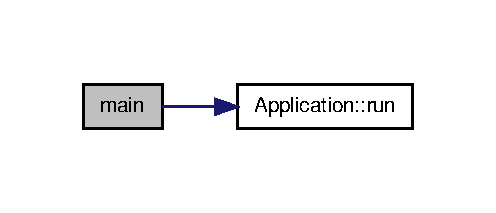
\includegraphics[width=238pt]{_main_8cpp_ae66f6b31b5ad750f1fe042a706a4e3d4_cgraph}
\end{center}
\end{figure}



\hypertarget{_utility_8cpp}{\section{/home/gabriel/\-Templates/\-Stereo\-Vision/\-Source/\-Utility.cpp File Reference}
\label{_utility_8cpp}\index{/home/gabriel/\-Templates/\-Stereo\-Vision/\-Source/\-Utility.\-cpp@{/home/gabriel/\-Templates/\-Stereo\-Vision/\-Source/\-Utility.\-cpp}}
}
{\ttfamily \#include $<$S\-V/\-Utility.\-hpp$>$}\\*
{\ttfamily \#include $<$iostream$>$}\\*
{\ttfamily \#include $<$fstream$>$}\\*
{\ttfamily \#include $<$ctime$>$}\\*
{\ttfamily \#include $<$cstdio$>$}\\*
{\ttfamily \#include $<$cstdlib$>$}\\*
{\ttfamily \#include $<$unistd.\-h$>$}\\*
{\ttfamily \#include $<$sys/types.\-h$>$}\\*
{\ttfamily \#include $<$sys/wait.\-h$>$}\\*
Include dependency graph for Utility.\-cpp\-:
\nopagebreak
\begin{figure}[H]
\begin{center}
\leavevmode
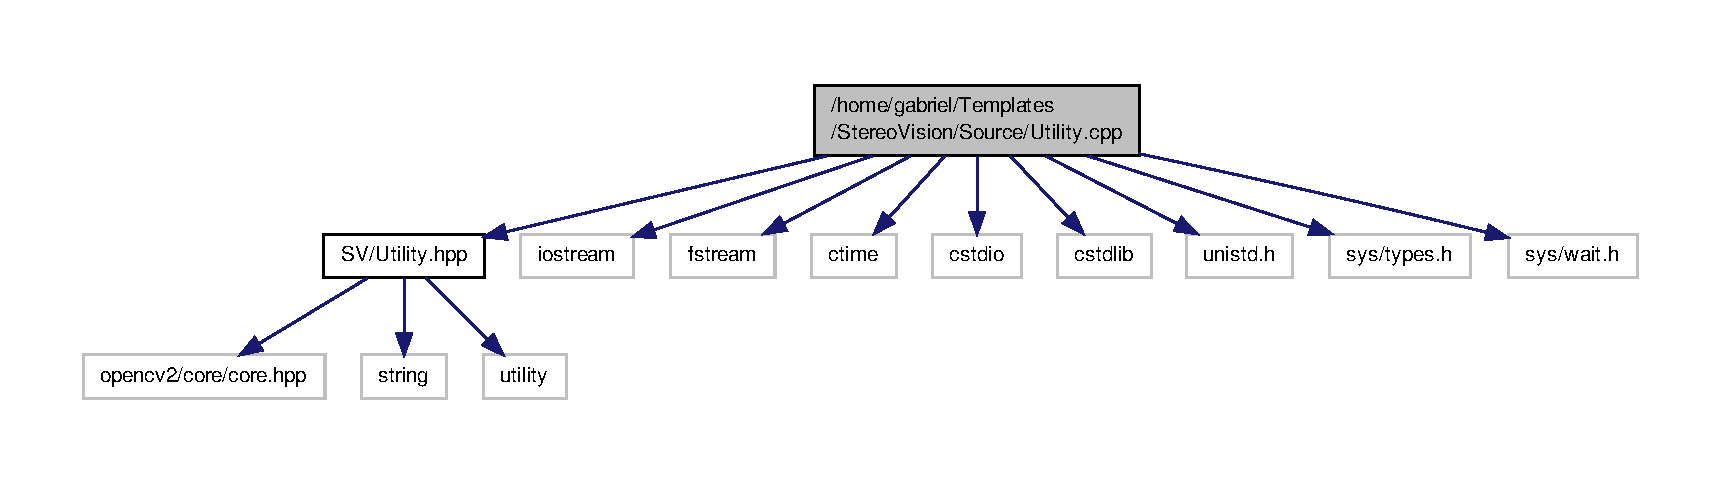
\includegraphics[width=350pt]{_utility_8cpp__incl}
\end{center}
\end{figure}

%--- End generated contents ---

% Index
\newpage
\phantomsection
\addcontentsline{toc}{part}{Index}
\printindex

\end{document}
